\documentclass{beamer}
\usepackage{booktabs}
\usepackage{pdfpages}
\usepackage{mathtools}
\usepackage{enumerate}
\usepackage{multirow,tabularx}
\usepackage{booktabs}
\usepackage{pdfpages}
\usepackage{proof}
\usepackage{cancel}
\usepackage{chronology}
\usepackage{graphicx}
\usepackage{ulem}
\usepackage{amsmath}
\usepackage{amssymb}
\usepackage{color}

\PassOptionsToPackage{usenames,dvipsnames,svgnames}{xcolor}  
\usepackage{tikz}
\usepackage{tkz-graph}


\usepackage{wasysym}
\usepackage{proof}
\usepackage{cancel}
\usepackage{chronology}
\usepackage{graphicx}
\usepackage{ulem}
\usepackage{amsmath}
\usepackage{amssymb}
\usepackage{color}
\usepackage{xcolor}
\usepackage{soul}
%\usepackage{pstricks}
\setbeamertemplate{navigation symbols}{}

\newcommand{\myul}[2][blue]{\sethlcolor{#1}\hl{#2}\setulcolor{black}}

\newcommand<>{\cunderline}[3]{\only<#1>{#3}\only<#2>{\underline{#3}}}
\newcommand<>{\cem}[3]{\only<#1>{#3}\only<#2>{\ul{#3}}}
\newcommand<>{\cgray}[3]{\only<#1>{#3}\only<#2>{\textcolor{gray}{#3}}}
\newcommand<>{\colorize}[4]{\only<#1>{#4}\only<#2>{\textcolor{#3}{#4}}}

%\setbeamertemplate{navigation symbols}{}
\addtobeamertemplate{navigation symbols}{}{%
    \usebeamerfont{footline}%
    \usebeamercolor[fg]{footline}%
    \hspace{1em}%
    \insertframenumber/\inserttotalframenumber
}

\renewcommand{\em}{\itshape}

\mode<presentation>
% {
%   \usecolortheme{crane}
% %  \usetheme{Frankfurt}
% }
\mode<presentation>
{
  \usecolortheme{dove}
}

% \mode<presentation>
% {
% \useinnertheme[shadow=true]{rounded}
% \useoutertheme{infolines}
% \usecolortheme{dove}
% \setbeamerfont{block title}{size={}}
% }

\title[Bio-Ontologies]{Introduction to ontologies in computational biology}

\author{Robert Hoehndorf}


\date{}

\begin{document}

\begin{frame}
  \titlepage
\end{frame}

% What ontologies are

% How to find ontology => excercise

% Axioms in ontologies => excercise in AberOWL

% OWL basics, and reasoning; OBO-style and OWL-style identifiers

% How ontologies are used; Gene Ontology; Phenotypes => excercise:
% find annotations


\begin{frame}
\frametitle{Overview}
\tableofcontents
\end{frame}

\section{General overview}

\begin{frame}
  \frametitle{Ontology (the discipline)}
  \begin{itemize}
  \item builds on philosophy, cognitive science, linguistics and logic
  \item with the purpose of understanding, clarifying, making explicit and
    communicating {\em people's assumptions} about the nature and
    structure of the world.
  \item orientation towards helping people (and machines) understand each other
    distinguishes applied ontology from philosophical ontology, and
    motivates its unavoidable interdisciplinary nature.
  \item Ontological analysis: study of content (of these assumptions)
    as such (independently of their representation)
  \end{itemize}
\end{frame}

\begin{frame}
  \frametitle{Kinds of knowledge}
  \begin{itemize}
  \item Fido is black: assertional
  \item Either Fido is black or Fido is not black: analytic, logical
  \item If Jack is a bachelor, then he is not married: analytic,
    terminological
    \begin{itemize}
    \item Terminological knowledge is about relationships between
      terms and concepts
    \end{itemize}
  \end{itemize}
\end{frame}

\begin{frame}
  \frametitle{What is an ontology?}
  \framesubtitle{Ontology: the philosophical discipline}
  \begin{itemize}
  \item Study of what there is (being {\em qua} being)
  \item reinterpreted for computer science: content {\em qua} content,
    independently of the way it is represented
  \item Study of the nature and structure of ``reality'' (a domain of discourse)
  \item A (philosophical) ontology: a structured system of entities assumed to exists,
    organized in categories and relations
  \end{itemize}
\end{frame}

\begin{frame}
  \frametitle{Ontologies in CS}
  \begin{itemize}
  \item Specific (theoretical or computational) artifacts expressing
    the intended meaning of a vocabulary in terms of primitive
    categories and relations describing the nature and structure of a
    domain of discourse 
    \begin{itemize}
    \item in order to account for the competent use of vocabulary in
      real situations
    \end{itemize}
  \end{itemize}
\end{frame}

\begin{frame}
  \frametitle{Ontologies in CS}
  \begin{itemize}
  \item Gruber: ``A specification of a conceptualization of a domain''
  \item Studer: ``An ontology is a formal, explicit specification of a
    shared conceptualization''
  \item Guarino: ``An ontology is a logical theory accounting for the
    intended meaning of a formal vocabulary, i.e. its ontological
    commitment to a particular conceptualization of the world. The
    intended models of a logical language using such a vocabulary are
    constrained by its ontological commitment. An ontology indirectly
    reflects this commitment (and the underlying conceptualization) by
    approximating these intended models.''
  \item Horrocks: ``an ontology [is] equivalent to a Description Logic
    knowledge base''
  \end{itemize}
\end{frame}

\begin{frame}
  \frametitle{What is a conceptualization}
  \begin{itemize}
  \item Formal structure of (a piece of) reality as perceived and organized by an
    agent, independently of:
    \begin{itemize}
    \item the vocabulary used
    \item the actual occurence of a specific situation
    \end{itemize}
  \item Different situations involving the same objects, described by
    different vocabularies, may share the same conceptualization
  \end{itemize}
\end{frame}

\begin{frame}
  \frametitle{Ontologies vs classifications}
  % Ontological analysis, slide 32
  \begin{itemize}
  \item Classifications focus on:
    \begin{itemize}
    \item access, based on pre-determined criteria (encoded by
      syntactic keys)
    \end{itemize}
  \item Ontologies focus on:
    \begin{itemize}
    \item meaning of terms
    \item nature and structure of a domain
    \end{itemize}
  \end{itemize}
\end{frame}

\begin{frame}
  \frametitle{Ontologies vs Knowledge bases}
  Knowledge base:
  \begin{itemize}
  \item Assertional component
    \begin{itemize}
    \item reflects specific states of affairs
    \item designed for problem solving
    \end{itemize}
  \item Terminological component (ontology)
    \begin{itemize}
    \item independent of states of affairs
    \item designed to support terminological services
    \item ... but independent of the actual terminology used
    \end{itemize}
  \item Ontological formulas are invariant, necessary information
    \begin{itemize}
    \item often expressed using modal logics or Description Logics
    \end{itemize}
  \end{itemize}
\end{frame}

\begin{frame}
  \frametitle{Ontologies}
  \begin{itemize}
  \item {\em classes} represent kinds of things in the world
    \begin{itemize}
    \item {\em Arm}, {\em Apoptosis}, {\em Influenza}, {\em Homo
        sapiens}, {\em Drinking behavior}, {\em Membrane}
    \end{itemize}
    \pause
  \item {\em instances} of classes are individuals satisfying the
    classes' intension
    \begin{itemize}
    \item my arm, the influenza I had last year, one ethanol molecule, etc.
    \end{itemize}
    \pause
  \item {\em relations} between instances arise from interactions,
    configurations, etc., of individuals
    \begin{itemize}
    \item my arm is {\bf part of} me, the {\bf duration of} my
      influenza was 10 days
    \end{itemize}
    \pause
  \item {\em axioms} specify the conditions that instances of a class
    must satisfy
    \begin{itemize}
    \item every instance of {\em Hand} is a {\bf part of} an instance
      of {\em Arm}
    \item axioms are specified using a formal language (logic)
    \end{itemize}
  \end{itemize}
\end{frame}

\begin{frame}
  \frametitle{Ontology repositories}
  \begin{itemize}
  \item BioPortal: \url{https://bioportal.bioontology.org/}
  \item Ontology Lookup Service: \url{https://www.ebi.ac.uk/ols/}
  \item OntoBee: \url{http://www.ontobee.org/}
  \item AberOWL: \url{http://aber-owl.net}
  \item OBO Foundry: \url{http://www.obofoundry.org/}
  \item AgroPortal: \url{http://agroportal.lirmm.fr/}
  \end{itemize}
\end{frame}

\begin{frame}
  \frametitle{Ontology repositories}
  Excercise:
  \begin{itemize}
  \item Find the ``Gene Ontology'' in BioPortal, OLS, and AberOWL
  \item Find the ``GO-PLUS'' ontology in AberOWL
  \item Find the Mammalian Phenotype (MP) ontology
  \item Find the class ``B cell apoptotic process'' in GO (or
    GO-PLUS); what are its identifiers?
  \item Find all the axioms pertaining to ``B cell apoptotic process''
  \item Find the class ``decreased B cell apoptosis'' in the MP; what
    are its identifiers and all the axioms?
  \end{itemize}
\end{frame}

\begin{frame}
  \frametitle{Ontologies and annotations}
  \begin{itemize}
  \item database integration through ontologies:
    \begin{itemize}
    \item shared classes, shared identifiers
    \item used in databases, websites, file downloads, etc.
    \end{itemize}
  \end{itemize}
\end{frame}

\begin{frame}
  \frametitle{Ontologies and annotations}
  Where to find ontology-based annotations:
  \begin{itemize}
  \item websites: AmiGO, model organism databases (MGI, ZFIN, FlyBase,
    ...), UniProt, etc.
  \item files: data files, GFF3,...
  \end{itemize}
\end{frame}

\begin{frame}
  \frametitle{Ontologies and annotations}
  Excercise:
  \begin{itemize}
  \item Use AmiGO and find all gene products in human associated with
    ``B cell apoptotic process''; notice the difference between
    ``direct'' and ``indirect'' annotations!
    \begin{itemize}
    \item \url{http://amigo.geneontology.org/amigo}
    \end{itemize}
  \item Download GO annotations in mouse
    (\url{http://www.informatics.jax.org/downloads/reports/index.html},
    {\tt gene\_association.mgi.gz})
    and find all gene products associated with ``B cell apoptotic
    process''
    \begin{itemize}
    \item notice the identifiers
    \item how to get ``indirect'' annotations?
    \end{itemize}
  \end{itemize}
\end{frame}

\section{Ontologies and the Semantic Web}
\begin{frame}
  \frametitle{The Semantic Web}
  \centerline{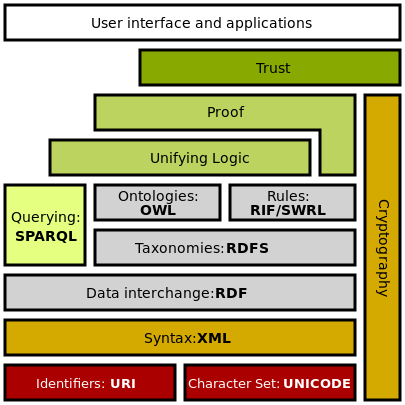
\includegraphics[width=.6\textwidth]{semwebstack.png}}
\end{frame}

\begin{frame}
  \frametitle{Web Ontology Language (OWL)}
  \begin{itemize}
  \item OWL 2 is based on the Description Logic $\mathcal{SROIQ(D)}$
  \item $\mathcal{ALC}$ with
    \begin{itemize}
    \item complex role inclusions: $r \circ s \subseteq r$
    \item role hierarchy: $r \subseteq s$
    \item role transitivity $r \circ r \subseteq r$
    \item nominals: $\{ a_1,...,a_n\}$ as concept constructor
    \item qualified number restrictions: $(\leq n r.Q)$
    \item datatype properties: $\exists r.[\geq n (Integer)]$
    \end{itemize}
  \end{itemize}
\end{frame}

% \begin{frame}
%   \frametitle{OWL subsets}
%   \begin{itemize}
%   \item OWL 2: $\mathcal{SROIQ(D)}$
%   \item OWL Lite: $\mathcal{SHIF(D)}$
%   \item OWL DL: $\mathcal{SHOIN(D)}$
%   \item OWL Full: non-standard semantics, undecidable
%   \item tractable subsets, OWL profiles:
%     \begin{itemize}
%     \item OWL EL
%     \item OWL RL
%     \item OWL QL
%     \end{itemize}
%   \end{itemize}
% \end{frame}

\begin{frame}
  \frametitle{Terminology}
  \begin{itemize}
  \item Instances
  \item Properties
    \begin{itemize}
    \item Object properties
    \item Datatype properties
    \end{itemize}
  \item Classes
  \item Meta-classes
    \begin{itemize}
    \item OWL Full
    \item Punning
    \end{itemize}
  \item Axiom
    \begin{itemize}
    \item Class axioms: Subclass, Equivalent class, Disjoint class
    \item Property axioms
    \end{itemize}
  \item Ontology
  \item OWL: Web Ontology Language
  \end{itemize}
\end{frame}

\begin{frame}
  \frametitle{Syntax}
  \begin{itemize}
  \item originally an extension of RDF and RDF Schema
  \item several different syntaxes
  \end{itemize}
  Consider the axiom $Parent \equiv Human \sqcap \exists hasChild.\top$
\end{frame}

\begin{frame}[fragile]
  \frametitle{Functional Syntax}
\begin{verbatim}
EquivalentClasses(:Parent 
  ObjectSomeValuesFrom(:hasChild owl:Thing))
\end{verbatim}
\end{frame}

\begin{frame}[fragile]
  \frametitle{RDF/XML Syntax}
{\tiny
\begin{verbatim}
    <owl:Class rdf:about="http://example.com/demo-ontology.owl#Parent">
        <owl:equivalentClass>
            <owl:Restriction>
                <owl:onProperty rdf:resource="http://example.com/demo-ontology.owl#hasChild"/>
                <owl:someValuesFrom rdf:resource="&owl;Thing"/>
            </owl:Restriction>
        </owl:equivalentClass>
    </owl:Class>
\end{verbatim}
}
\end{frame}

\begin{frame}[fragile]
  \frametitle{RDF Turtle Syntax}
{\tiny
\begin{verbatim}
:Parent rdf:type owl:Class ;
        
        owl:equivalentClass [ rdf:type owl:Restriction ;
                              owl:onProperty :hasChild ;
                              owl:someValuesFrom owl:Thing
                            ] .
\end{verbatim}
}
\end{frame}

\begin{frame}[fragile]
  \frametitle{OWL/XML Syntax}
{\tiny
\begin{verbatim}
    <EquivalentClasses>
        <Class IRI="#Parent"/>
        <ObjectSomeValuesFrom>
            <ObjectProperty IRI="#hasChild"/>
            <Class abbreviatedIRI="owl:Thing"/>
        </ObjectSomeValuesFrom>
    </EquivalentClasses>
\end{verbatim}
}
\end{frame}

\begin{frame}[fragile]
  \frametitle{Manchester OWL Syntax}
{\tiny
\begin{verbatim}
Class: Parent
    EquivalentTo: 
        hasChild some owl:Thing
\end{verbatim}
}
\end{frame}

\begin{frame}
  \frametitle{Manchester OWL Syntax}
  \begin{table}[ht]
    \centering
    \begin{tabular}{|l|l|l|}
      DL Syntax & Manchester Syntax & Example \\
      \hline
      $C \sqcap D$ & C and D & Human and Male \\
      $C \sqcup D$ & C or D & Male or Female \\
      $\neg C$ & not C & not Male \\
      $\exists R.C$ & R some C & hasChild some Human \\
      $\forall R.C$ & R only C & hasChild only Human \\
      $(\geq n R.C)$ & R min n C & hasChild min 1 Human \\
      $(\leq n R.C)$ & R max n C & hasChild max 1 Human \\
      $(= n R.C)$ & R exactly n C & hasChild exactly 1 Human \\
      $\{a\} \sqcup \{b\} \sqcup ...$ & \{a b ...\} & \{John Robert
                                                      Mary\} \\
      \hline
    \end{tabular}
  \end{table}
\end{frame}

\begin{frame}[fragile]
  \frametitle{OWL classes and namespaces}
  \begin{itemize}
  \item $\bot$ is {\tt owl:Nothing}
  \item $\top$ is {\tt owl:Thing}
  \item {\tt owl:} is a {\em namespace}
    (\url{http://www.w3.org/2002/07/owl#})
  \item {\tt owl:Thing} expands to {\tt
      http://www.w3.org/2002/07/owl\#Thing} (a class IRI)
  \item all OWL entities (ontologies, classes, properties, instances)
    are referred to by an IRI
  \item namespaces define a common (IRI-)prefix, e.g.,
    \begin{itemize}
    \item {\tt rdf:} {\tt http://www.w3.org/1999/02/22-rdf-syntax-ns\#}
    \item {\tt rdfs:} {\tt http://www.w3.org/2000/01/rdf-schema\#}
    \end{itemize}
  \item can define own namespaces:
{\tiny
\begin{verbatim}
Namespace: mynamespace <http://www.kaust.edu.sa#>
Class: mynamespace:Student # http://www.kaust.edu.sa#Student
\end{verbatim}
}
  \end{itemize}
\end{frame}

\begin{frame}
  \frametitle{Object properties}
  \begin{itemize}
  \item Object property characteristics:
    \begin{itemize}
    \item transitive
    \item symmetric, asymmetric
    \item reflexive, irreflexive
    \item functional, inverse functional
    \item inverse of
    \end{itemize}
  \item Domain and range
  \end{itemize}
\end{frame}

\begin{frame}
  \frametitle{Annotation properties}
  \begin{itemize}
  \item OWL entities (classes, properties, axioms, ontologies, etc.)
    can have {\em annotations}
  \item outside of OWL semantics (unless for OWL Full)
  \item useful to add labels, synonyms, explanation, (textual)
    definitions, authoring information, versions, etc.
  \item predefined: {\tt rdfs:label}, {\tt owl:versionInfo}, {\tt
      rdfs:comment}, {\tt rdfs:seeAlso}, {\tt rdfs:isDefinedBy}
  \item Dublin Core
  \end{itemize}
\end{frame}

\begin{frame}
  \frametitle{OWL Reasoning}
  \begin{itemize}
  \item Classification: compute the most specific sub- and
    super-classes for each named class in an OWL ontology
  \item Subsumption: find all sub-, super- or equivalent classes of an
    OWL class description
  \item Consistency: find contradictions in OWL knowledge base
  \item Instantiation: is $a$ and instance of $C$?
  \end{itemize}
\end{frame}

\begin{frame}
  \frametitle{Complexity of reasoning in OWL}
  \begin{itemize}
  \item OWL 2 ($\mathcal{SROIQ}$) is 2NEXPTIME-complete
  \item OWL (1) ($\mathcal{SHOIN}$) is NEXPTIME-complete
  \item OWL Lite ($\mathcal{SHIF}$) is EXPTIME-complete
  \end{itemize}
  \vspace{2cm}
\end{frame}

\begin{frame}
  \frametitle{OWL profiles}
  \begin{itemize}
  \item OWL 2 EL: PTIME-complete
  \item OWL 2 RL: PTIME-complete
  \item OWL 2 QL: $AC^0$ w.r.t. data size
  \end{itemize}
\end{frame}

\begin{frame}
  \frametitle{OWL 2 EL}
  \begin{itemize}
  \item Class axioms:
    \begin{itemize}
    \item subclass, equivalent class, disjoint class
    \end{itemize}
  \item Object property axioms:
    \begin{itemize}
    \item domain and range restrictions, property inclusion, property
      chains, property equivalence, transitive and reflexive properties
    \end{itemize}
  \item Class descriptions:
    \begin{itemize}
    \item intersection, existential quantification, enumerations to a
      single individual
    \end{itemize}
  \item Assertions: all
  \end{itemize}
\end{frame}

\begin{frame}
  \frametitle{Why OWL?}
  \begin{itemize}
  \item OWL exploits 20+ years of research on Description Logic
  \item well-defined semantics
  \item complexity and decidability well understood
  \item known algorithms
  \item scalability demonstrated in practise
  \end{itemize}
\end{frame}

\begin{frame}
  \frametitle{Why OWL?}
  Major benefit is the large number of tools and infrastructure:
  \begin{itemize}
  \item Editors: Protege, WebProtege
  \item Reasoners: HermiT, Pellet, FaCT++, {\bf ELK}, KAON2, RACER,...
  \item Explanation, justification
  \item Modularization
  \item APIs (esp. the OWL API)
  \end{itemize}
\end{frame}

\begin{frame}
  \frametitle{OWL vs Databases}
  \begin{table}[ht]
    \centering
    \begin{tabular}{|l|l|}
      Database & OWL Ontology \\
      \hline
      Closed World Assumption & Open World Assumption \\
      Unique Name Assumption & No UNA \\
      Schema constraints data structure %, defining legal states of
                                %the database 
               & Axioms behave like inference rules\\\hline
    \end{tabular}
  \end{table}
\end{frame}

\begin{frame}
  \frametitle{Examples: OWL vs Databases}
  {\tiny Based on slides by Ian Horrocks}
  \vfill
  \begin{itemize}
  \item hasPet some owl:Thing SubclassOf: Human
  \item Phoenix SubclassOf: petOf only Wizard
  \item HarryPotter: Wizard
  \item DracoMalfoy: Wizard
  \item HarryPotter hasFriend RonWeasley
  \item HarryPotter hasFriend HermioneGranger
  \item HarryPotter hasPet Hedwig
  \end{itemize}
  Query: Is Draco a friend of Harry Potter?
  \pause
  \begin{itemize}
  \item DB: No
  \item OWL: Don't know
  \end{itemize}
\end{frame}

\begin{frame}
  \frametitle{Examples: OWL vs Databases}
  \begin{itemize}
  \item hasPet some owl:Thing SubclassOf: Human
  \item Phoenix SubclassOf: petOf only Wizard
  \item HarryPotter: Wizard
  \item DracoMalfoy: Wizard
  \item HarryPotter hasFriend RonWeasley
  \item HarryPotter hasFriend HermioneGranger
  \item HarryPotter hasPet Hedwig
  \end{itemize}
  Query: How many friends has Harry Potter?
  \pause
  \begin{itemize}
  \item DB: 2
  \item OWL: At least 1
  \end{itemize}
\end{frame}

\begin{frame}
  \frametitle{Examples: OWL vs Databases}
  \begin{itemize}
  \item hasPet some owl:Thing SubclassOf: Human
  \item Phoenix SubclassOf: petOf only Wizard
  \item HarryPotter: Wizard
  \item DracoMalfoy: Wizard
  \item HarryPotter hasFriend RonWeasley
  \item HarryPotter hasFriend HermioneGranger
  \item HarryPotter hasPet Hedwig
  \item RonWeasley $\not=$ HermioneGranger
  \item HarryPotter: hasFriend only \{HerminoeGranger RonWeasley\}
  \end{itemize}
  Query: How many friends has Harry Potter?
  \pause
  \begin{itemize}
  \item DB: 2
  \item OWL: 2
  \end{itemize}
\end{frame}

\begin{frame}
  \frametitle{Examples: OWL vs Databases}
  \begin{itemize}
  \item hasPet some owl:Thing SubclassOf: Human
  \item Phoenix SubclassOf: petOf only Wizard
  \end{itemize}
  Adding new facts:
  \begin{itemize}
  \item Dumbledore: Wizard
  \item Fawkes: Phoenix
  \item Fawkes isPetOf DumbleDore
  \end{itemize}
  \begin{itemize}
  \item DB: Update rejects, constrain violation
  \item OWL: infer that Dumbledore is Human; infer that Dumbledore is
    a Wizard
  \end{itemize}
\end{frame}

\begin{frame}
  \frametitle{Ontology-based information systems}
  Ontology like DB schema, instances like data\\
  Advantages:
  \begin{itemize}
  \item Relatively easy to maintain and update schema
  \item Query answers reflect both schema and data
  \item Can deal with incomplete information
  \item Answer intensional and extensional queries
  \end{itemize}
  Disadvantages:
  \begin{itemize}
  \item Semantic can seem counter-intuitive (OWA, UNA)
  \item Query answering (logical entailment) much more difficult
  \end{itemize}
\end{frame}

\section{Ontologies and graphs}

\begin{frame}
  \frametitle{Some examples}
  \begin{itemize}
  \item Are cyclin dependent kinases {\em functionally} more similar
    to lipid kinases or to riboflavin kinases? How about {\em
      phenotypically}?
    \pause
  \item Which protein in the {\em mouse} is functionally most similar
    to the zebrafish {\em gustducin} protein?
    \pause
  \item Which mouse knockout resembles {\em Bardet-Biedl Syndrome 8}?
    \pause
  \item Are there mouse knockouts that resemble the side effects of
    diclofenac?
    \pause
  \item Which genetic disease produces similar symptoms to ebola?
    \pause
  \item Does functional similarity correlate with phenotypic similarity?
  \end{itemize}
\end{frame}

\begin{frame}
  \frametitle{Ontologies and graphs}
  \begin{itemize}
  \item semantic similarity measures can be graph-based,
    feature-based, or model-based
  \item we may need to generate graphs from ontologies
    \begin{itemize}
    \item {\em is-a} relations are easy
    \item how about {\em part-of}, {\em regulates}, {\em precedes}, etc.?
    \end{itemize}
  \item relational patterns are implicit in OWL axioms
    \begin{itemize}
    \item in first order logic
    \item needs to translate them into OWL
    \item defined in OBO Relation Ontology
    \end{itemize}
  \end{itemize}
\end{frame}

\begin{frame}
  \frametitle{Relations as patterns}
  \begin{itemize}
  \item {\tt X SubClassOf: Y}: $X \xrightarrow{\text{is-a}} Y$
  \item {\tt X SubClassOf: part-of some Y}: $X \xrightarrow{\text{part-of}} Y$
  \item {\tt X SubClassOf: regulates some Y}: $X \xrightarrow{\text{regulates}} Y$
  \item {\tt X DisjointWith: Y}: $X \xleftrightarrow{\text{disjoint}} Y$
  \item {\tt X EquivalentTo: Y}: $X \xleftrightarrow{\equiv} Y$, $\{X,Y\}$
  \end{itemize}
\end{frame}

\begin{frame}
  \frametitle{Relations as patterns}
  \begin{itemize}
  \item OBO Relation Ontology (RO):
    \begin{itemize}
    \item \url{https://github.com/oborel/obo-relations}
    \end{itemize}
  \item Basic Formal Ontology (BFO):
    \begin{itemize}
    \item provides top-level classes
      \begin{itemize}
      \item Continuant, Process, Function, Material object, etc.
      \end{itemize}
    \item used for some OBO Foundry ontologies
    \end{itemize}
  \item RO and BFO provide a top-level system of classes and relations
    shared across many biomedical ontologies
    \begin{itemize}
    \item even GO, although somewhat hidden!
    \end{itemize}
  \end{itemize}
\end{frame}

\begin{frame}
  \frametitle{Relations as patterns}
  \centerline{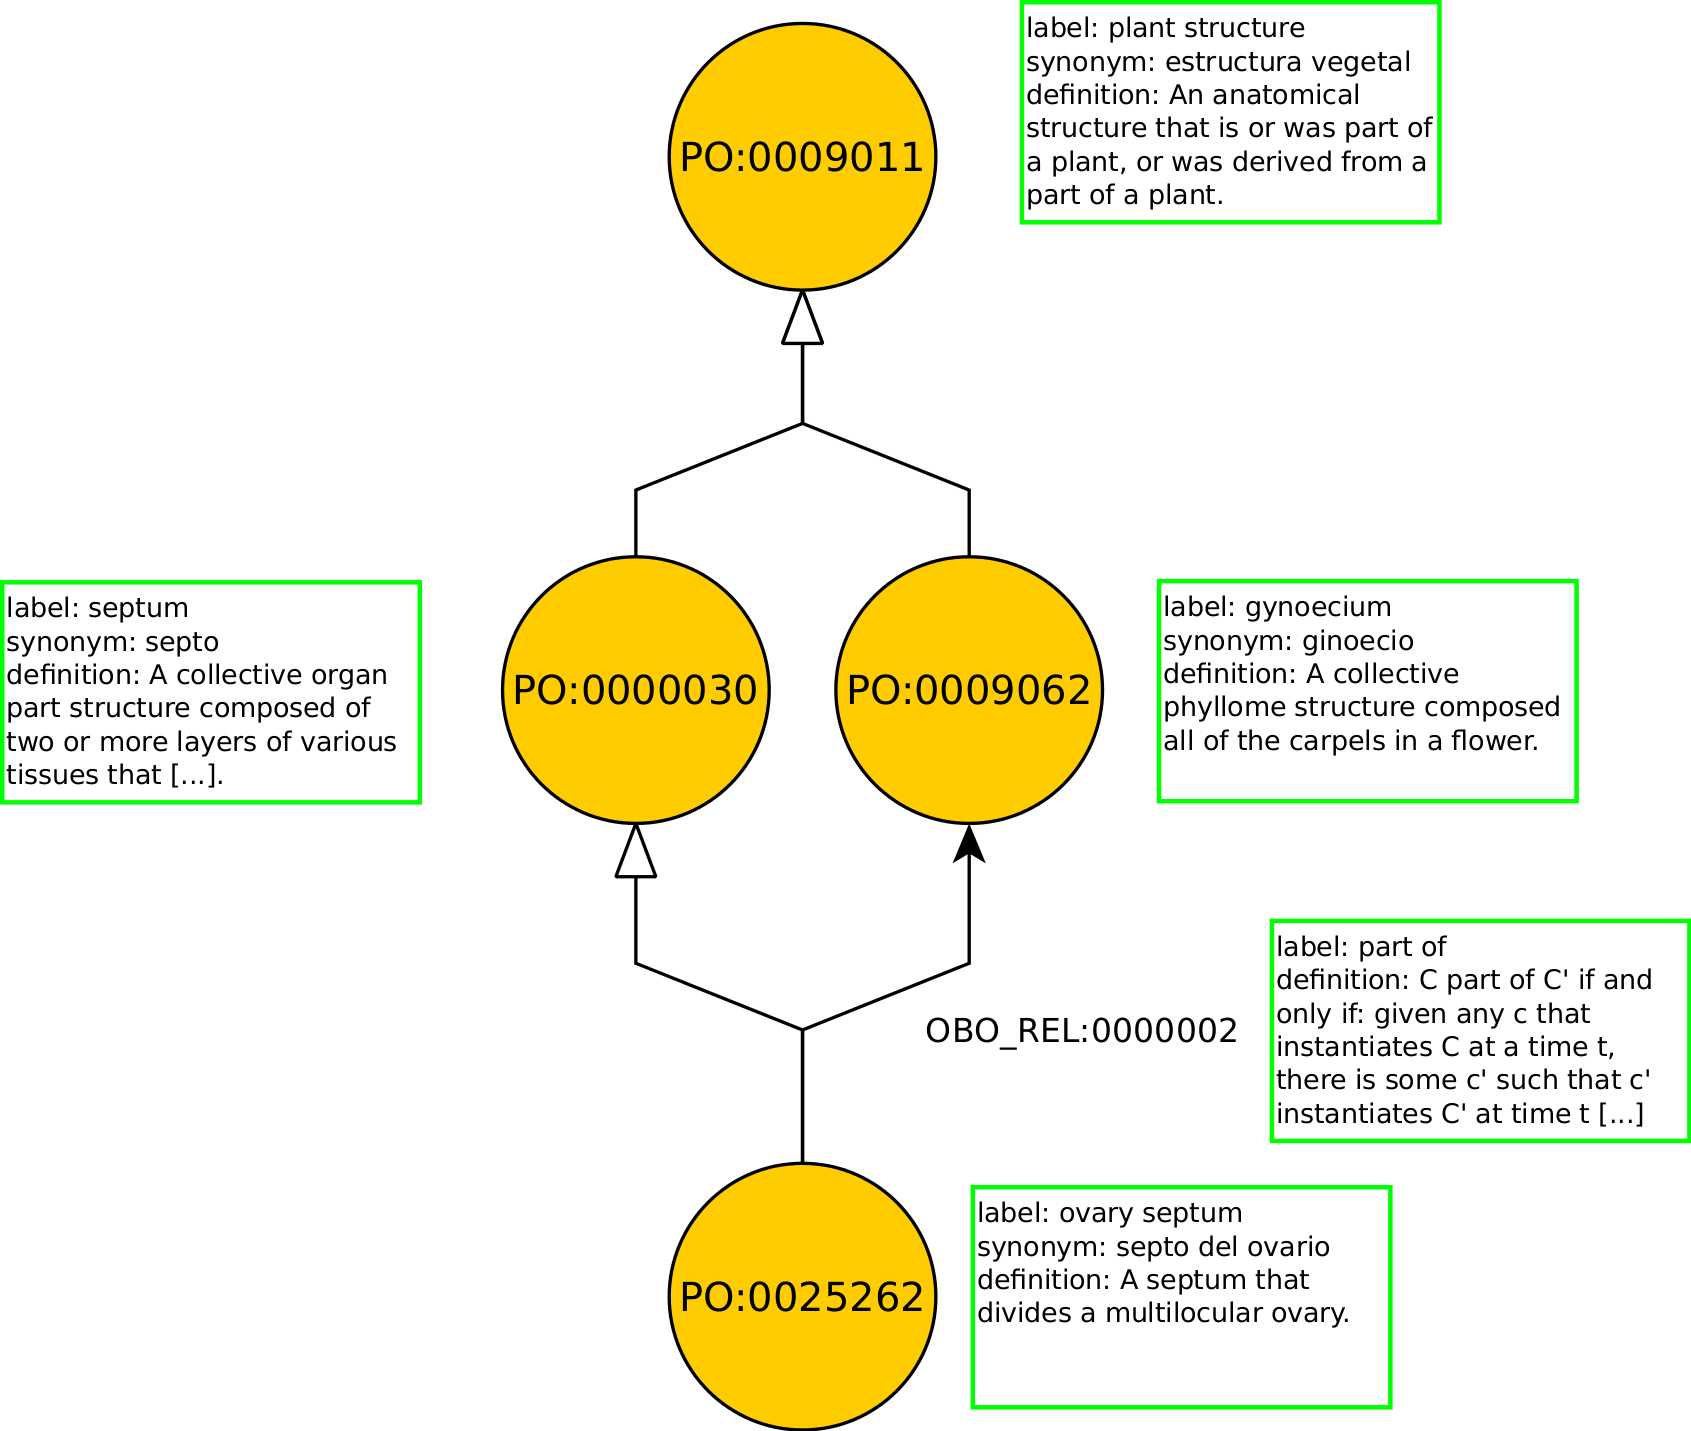
\includegraphics[height=.8\textheight]{plant-ontology-sample.png}}
\end{frame}

\begin{frame}
  \frametitle{Relations as patterns: Quiz}
  \begin{itemize}
  \item {\em classes}
    \begin{enumerate}[a]
    \item represent kinds of things in the world
    \item represent ideas in people's heads
    \item represent words
    \end{enumerate}
    \pause
  \item {\em instances} of a class are individuals that
    \begin{enumerate}[a]
    \item satisfy the class intension
    \item satisfy the axioms used to specify the class
    \item are always concrete, material entities
    \end{enumerate}
    \pause
  \item {\em relations between classes} are
    \begin{enumerate}[a]
    \item interactions between instances of the class
    \item abbreviations of axioms that constrain two classes
    \item relations between ideas people have about the classes
    \end{enumerate}
    \pause
  \item {\em axioms} are
    \begin{enumerate}[a]
    \item specification of conditions that instances of classes must satisfy
    \item rules that can be executed to produce new knowledge
    \item statements that are considered to be true in a domain of knowledge
    \end{enumerate}
  \end{itemize}
\end{frame}

\section{Semantic Similarity}

\begin{frame}
  \frametitle{How to measure similarity?}
  \begin{itemize}
  \item semantic similarity measures similarity between classes
  \item semantic similarity measures similarity between instances of classes
  \item semantic similarity measures similarity between entities
    annotated with classes
  \item $\Rightarrow$ reduce all of this to similarity between classes
  \end{itemize}
\end{frame}

\begin{frame}
  \frametitle{How to measure similarity?}
  What properties do we want in a similarity measure?
  \\
  A function $sim: D \times D$ is a similarity on $D$ if, for
  all $x, y \in D$, the function $sim$ is:  \begin{itemize}
    \pause
  \item non-negative: $sim(x,y) \geq 0$ for all $x, y$
    \pause
  \item symmetric: $sim(x,y) = sim(y,x)$
    \pause
  \item reflexive: $sim(x,x) = max_D$
    \pause
    \begin{itemize}
    \item weaker form: $sim(x,x) > sim(x,y)$ for all $x \not= y$
    \end{itemize}
    \pause
  \item $sim(x,x) > sim(x,y)$ for $x\not= y$
    \pause
  \item $sim$ is a {\em normalized} similarity measure if it has
    values in $[0,1]$
  \end{itemize}
\end{frame}

\usetikzlibrary{arrows,positioning,automata}
\begin{frame}
  \frametitle{How to measure similarity?}
  \begin{columns}
    \begin{column}{.6\textwidth}
      {\tiny
        \begin{tikzpicture}[>=stealth',shorten >=1pt,node distance=2cm,on grid,initial/.style    ={}]
          \node[state]          (A)                        {$Thing$};
          \node[state]          (B) [below left =of A]    {$Color$};
          \node[state]          (C) [below right =of A]    {$Shape$};
          \node[state]          (D) [below left =of B]    {$Red$};
          \node[state]          (H) [below right =of B]    {$Green$};
          \node[state]          (E) [below  =of D]    {$Orange$};
          \node[state]          (F) [below =of C]    {$Round$};
          \node[state]          (G) [below right =of C]    {$Square$};
          \tikzset{mystyle/.style={->,double=orange}} 
          \tikzset{every node/.style={fill=white}} 
          \path (B)     edge [mystyle]    node   {$isa$} (A)
          (C)     edge [mystyle]    node   {$isa$} (A) 
          (D)     edge [mystyle]    node   {$isa$} (B)
          (H)     edge [mystyle]    node   {$isa$} (B)
          (E)     edge [mystyle]    node   {$isa$} (D)
          (F)     edge [mystyle]    node   {$isa$} (C)
          (G)     edge [mystyle]    node   {$isa$} (C);
          \tikzset{mystyle/.style={<->,double=orange}}   
          \tikzset{mystyle/.style={<->,relative=true,in=0,out=60,double=orange}}
        \end{tikzpicture}
      }
    \end{column}
    \begin{column}{.4\textwidth}
      \begin{itemize}
        \pause
      \item distance on shortest path (Rada {\em et al.}, 1989)
        \pause
      \item $dist_{Rada}(u,v) = sp(u, isa, v)$
        \pause
      \item $sim_{Rada}(u,v) = \frac{1}{dist_{Rada}(u,v) + 1}$
      \end{itemize}
    \end{column}
  \end{columns}
\end{frame}

\begin{frame}
  \frametitle{How to measure similarity?}
  \begin{columns}
    \begin{column}{.6\textwidth}
      {\tiny
        \begin{tikzpicture}[>=stealth',shorten >=1pt,node distance=2cm,on grid,initial/.style    ={}]
          \node[state]          (A)                        {$Thing$};
          \node[state]          (B) [below left =of A]    {$Color$};
          \node[state]          (C) [below right =of A]    {$Shape$};
          \node[state, fill=green]          (D) [below left =of B]    {$Red$};
          \node[state, fill=green]          (H) [below right =of B]    {$Green$};
          \node[state]          (E) [below  =of D]    {$Orange$};
          \node[state]          (F) [below =of C]    {$Round$};
          \node[state]          (G) [below right =of C]    {$Square$};
          \tikzset{mystyle/.style={->,double=orange}} 
          \tikzset{highlight/.style={->,double=green}} 
          \tikzset{every node/.style={fill=white}}
          \path (B)     edge [mystyle]    node   {$isa$} (A)
          (C)     edge [mystyle]    node   {$isa$} (A) 
          (D)     edge [highlight]    node   {$isa$} (B)
          (H)     edge [highlight]    node   {$isa$} (B)
          (E)     edge [mystyle]    node   {$isa$} (D)
          (F)     edge [mystyle]    node   {$isa$} (C)
          (G)     edge [mystyle]    node   {$isa$} (C);
          \tikzset{mystyle/.style={<->,double=orange}}   
          \tikzset{mystyle/.style={<->,relative=true,in=0,out=60,double=orange}}
        \end{tikzpicture}
      }
    \end{column}
    \begin{column}{.4\textwidth}
      \begin{itemize}
      \item distance on shortest path
        \pause
       \item distance(green, red) = 2
       \item $sim_{Rada}(green, red) = \frac{1}{3}$
      \end{itemize}
    \end{column}
  \end{columns}
\end{frame}

\begin{frame}
  \frametitle{How to measure similarity?}
  \begin{columns}
    \begin{column}{.6\textwidth}
      {\tiny
        \begin{tikzpicture}[>=stealth',shorten >=1pt,node distance=2cm,on grid,initial/.style    ={}]
          \node[state]          (A)                        {$Thing$};
          \node[state]          (B) [below left =of A]    {$Color$};
          \node[state]          (C) [below right =of A]    {$Shape$};
          \node[state]          (D) [below left =of B]    {$Red$};
          \node[state]          (H) [below right =of B]    {$Green$};
          \node[state]          (E) [below  =of D]    {$Orange$};
          \node[state, fill=green]          (F) [below =of C]    {$Round$};
          \node[state, fill=green]          (G) [below right =of C]    {$Square$};
          \tikzset{mystyle/.style={->,double=orange}} 
          \tikzset{highlight/.style={->,double=green}} 
          \tikzset{every node/.style={fill=white}}
          \path (B)     edge [mystyle]    node   {$isa$} (A)
          (C)     edge [mystyle]    node   {$isa$} (A) 
          (D)     edge [mystyle]    node   {$isa$} (B)
          (H)     edge [mystyle]    node   {$isa$} (B)
          (E)     edge [mystyle]    node   {$isa$} (D)
          (F)     edge [highlight]    node   {$isa$} (C)
          (G)     edge [highlight]    node   {$isa$} (C);
          \tikzset{mystyle/.style={<->,double=orange}}   
          \tikzset{mystyle/.style={<->,relative=true,in=0,out=60,double=orange}}
        \end{tikzpicture}
      }
    \end{column}
    \begin{column}{.4\textwidth}
      \begin{itemize}
       \item distance on shortest path
       \item distance(square, round) = 2
       \item $sim_{Rada}(square, round) = \frac{1}{3}$
      \end{itemize}
    \end{column}
  \end{columns}
\end{frame}

\begin{frame}
  \frametitle{How to measure similarity?}
  \begin{columns}
    \begin{column}{.6\textwidth}
      {\tiny
        \begin{tikzpicture}[>=stealth',shorten >=1pt,node distance=2cm,on grid,initial/.style    ={}]
          \node[state]          (A)                        {$Thing$};
          \node[state, fill=green]          (B) [below left =of A]    {$Color$};
          \node[state]          (C) [below right =of A]    {$Shape$};
          \node[state]          (D) [below left =of B]    {$Red$};
          \node[state]          (H) [below right =of B]    {$Green$};
          \node[state, fill=green]          (E) [below  =of D]    {$Orange$};
          \node[state]          (F) [below =of C]    {$Round$};
          \node[state]          (G) [below right =of C]    {$Square$};
          \tikzset{mystyle/.style={->,double=orange}} 
          \tikzset{highlight/.style={->,double=green}} 
          \tikzset{every node/.style={fill=white}}
          \path (B)     edge [mystyle]    node   {$isa$} (A)
          (C)     edge [mystyle]    node   {$isa$} (A) 
          (D)     edge [highlight]    node   {$isa$} (B)
          (H)     edge [mystyle]    node   {$isa$} (B)
          (E)     edge [highlight]    node   {$isa$} (D)
          (F)     edge [mystyle]    node   {$isa$} (C)
          (G)     edge [mystyle]    node   {$isa$} (C);
          \tikzset{mystyle/.style={<->,double=orange}}   
          \tikzset{mystyle/.style={<->,relative=true,in=0,out=60,double=orange}}
        \end{tikzpicture}
      }
    \end{column}
    \begin{column}{.4\textwidth}
      \begin{itemize}
       \item distance on shortest path
       \item distance(orange, color) = 2
       \item $sim_{Rada}(orange, color) = \frac{1}{3}$
      \end{itemize}
    \end{column}
  \end{columns}
\end{frame}

\begin{frame}
  \frametitle{How to measure similarity?}
  \begin{itemize}
  \item shortest path is not always intuitive
    \pause
  \item we need a way to determine {\em specificity} of a class
    \begin{itemize}
    \item number of ancestors
    \item number of children
    \item information content
    \end{itemize}
    \pause
  \item {\em density} of a branch in the ontology
    \begin{itemize}
    \item number of siblings
    \item information content
    \end{itemize}
    \pause
  \item account for different edge types
    \begin{itemize}
    \item non-uniform edge weighting
    \end{itemize}
  \end{itemize}
\end{frame}

\begin{frame}
  \frametitle{How to measure similarity}
  \begin{itemize}
  \item term specificity measure $\sigma: C \mapsto \mathbb{R}$:
    \begin{itemize}
    \item $x \sqsubseteq y \rightarrow \sigma(x) \geq \sigma(y)$
    \end{itemize}
    \pause
  \item intrinsic:
    \begin{itemize}
    \item $\sigma(x) = f(depth(x))$
    \item $\sigma(x) = f(A(x))$ (for ancestors $A(x)$)
    \item $\sigma(x) = f(D(x))$ (for descendants $D(x)$)
    \item many more, e.g., Zhou et al.: $\sigma(x) = k \cdot \Big( 1-\frac{\log
        |D(x)|}{\log |C|} \Big) + (1-k) \frac{\log depth(x)}{\log
        depth(G_T)} $
    \end{itemize}
    \pause
  \item extrinsic:
    \begin{itemize}
    \item $\sigma(x)$ defined as a function of instances (or annotations) $I$
      \begin{itemize}
      \item note: the number of instances monotonically decreases with
        increasing depth in taxonomies
      \end{itemize}
    \item Resnik 1995: $eIC_{Resnik}(x) = -\log p(x)$ (with $p(x) =
      \frac{|I(x)|}{|I|}$)
      \begin{itemize}
      \item in biology, one of the most popular specificity measure when
        annotations are present
      \end{itemize}
    \end{itemize}
  \end{itemize}
\end{frame}

\begin{frame}
  \frametitle{How to measure similarity?}
  \begin{columns}
    \begin{column}{.6\textwidth}
      {\tiny
        \begin{tikzpicture}[>=stealth',shorten >=1pt,node distance=2cm,on grid,initial/.style    ={}]
          \node[state,label=below:$0.0$]          (A)                        {$Thing$};
          \node[state,label=below:$1.0$]          (B) [below left =of A]    {$Color$};
          \node[state,label=right:$1.0$]          (C) [below right =of A]    {$Shape$};
          \node[state,label=right:$2.0$]          (D) [below left =of B]    {$Red$};
          \node[state,label=below:$2.0$]          (H) [below right =of B]    {$Green$};
          \node[state,label=below:$3.0$]          (E) [below  =of D]    {$Orange$};
          \node[state,label=below:$2.0$]          (F) [below =of C]    {$Round$};
          \node[state,label=below:$2.0$]          (G) [below right =of C]    {$Square$};
          \tikzset{mystyle/.style={->,double=orange}} 
          \tikzset{highlight/.style={->,double=green}} 
          \tikzset{every node/.style={fill=white}}
          \path (B)     edge [mystyle]    node   {$isa$} (A)
          (C)     edge [mystyle]    node   {$isa$} (A) 
          (D)     edge [mystyle]    node   {$isa$} (B)
          (H)     edge [mystyle]    node   {$isa$} (B)
          (E)     edge [mystyle]    node   {$isa$} (D)
          (F)     edge [mystyle]    node   {$isa$} (C)
          (G)     edge [mystyle]    node   {$isa$} (C);
          \tikzset{mystyle/.style={<->,double=orange}}   
          \tikzset{mystyle/.style={<->,relative=true,in=0,out=60,double=orange}}
        \end{tikzpicture}
      }
    \end{column}
    \begin{column}{.4\textwidth}
      \begin{itemize}
      \item Resnik 1995: similarity between $x$ and $y$ is the
        information content of the {\em most informative common
          ancestor}
      \end{itemize}
    \end{column}
  \end{columns}
\end{frame}

\begin{frame}
  \frametitle{How to measure similarity?}
  \begin{columns}
    \begin{column}{.6\textwidth}
      {\tiny
        \begin{tikzpicture}[>=stealth',shorten >=1pt,node distance=2cm,on grid,initial/.style    ={}]
          \node[state,label=below:$0.0$]          (A)                        {$Thing$};
          \node[state,label=below:$1.0$]          (B) [below left =of A]    {$Color$};
          \node[state,label=right:$1.0$]          (C) [below right =of A]    {$Shape$};
          \node[state,fill=green,label=right:$2.0$]          (D) [below left =of B]    {$Red$};
          \node[state,fill=green,label=below:$2.0$]          (H) [below right =of B]    {$Green$};
          \node[state,label=below:$3.0$]          (E) [below  =of D]    {$Orange$};
          \node[state,label=below:$2.0$]          (F) [below =of C]    {$Round$};
          \node[state,label=below:$2.0$]          (G) [below right =of C]    {$Square$};
          \tikzset{mystyle/.style={->,double=orange}} 
          \tikzset{highlight/.style={->,double=green}} 
          \tikzset{every node/.style={fill=white}}
          \path (B)     edge [mystyle]    node   {$isa$} (A)
          (C)     edge [mystyle]    node   {$isa$} (A) 
          (D)     edge [mystyle]    node   {$isa$} (B)
          (H)     edge [mystyle]    node   {$isa$} (B)
          (E)     edge [mystyle]    node   {$isa$} (D)
          (F)     edge [mystyle]    node   {$isa$} (C)
          (G)     edge [mystyle]    node   {$isa$} (C);
          \tikzset{mystyle/.style={<->,double=orange}}   
          \tikzset{mystyle/.style={<->,relative=true,in=0,out=60,double=orange}}
        \end{tikzpicture}
      }
    \end{column}
    \begin{column}{.4\textwidth}
      \begin{itemize}
      \item Resnik 1995: similarity between $x$ and $y$ is the
        information content of the {\em most informative common
          ancestor}
      \end{itemize}
    \end{column}
  \end{columns}
\end{frame}

\begin{frame}
  \frametitle{How to measure similarity?}
  \begin{columns}
    \begin{column}{.6\textwidth}
      {\tiny
        \begin{tikzpicture}[>=stealth',shorten >=1pt,node distance=2cm,on grid,initial/.style    ={}]
          \node[state,label=below:$0.0$]          (A)                        {$Thing$};
          \node[state,fill=yellow,label=below:$1.0$]          (B) [below left =of A]    {$Color$};
          \node[state,label=right:$1.0$]          (C) [below right =of A]    {$Shape$};
          \node[state,fill=green,label=right:$2.0$]          (D) [below left =of B]    {$Red$};
          \node[state,fill=green,label=below:$2.0$]          (H) [below right =of B]    {$Green$};
          \node[state,label=below:$3.0$]          (E) [below  =of D]    {$Orange$};
          \node[state,label=below:$2.0$]          (F) [below =of C]    {$Round$};
          \node[state,label=below:$2.0$]          (G) [below right =of C]    {$Square$};
          \tikzset{mystyle/.style={->,double=orange}} 
          \tikzset{highlight/.style={->,double=green}} 
          \tikzset{every node/.style={fill=white}}
          \path (B)     edge [mystyle]    node   {$isa$} (A)
          (C)     edge [mystyle]    node   {$isa$} (A) 
          (D)     edge [mystyle]    node   {$isa$} (B)
          (H)     edge [mystyle]    node   {$isa$} (B)
          (E)     edge [mystyle]    node   {$isa$} (D)
          (F)     edge [mystyle]    node   {$isa$} (C)
          (G)     edge [mystyle]    node   {$isa$} (C);
          \tikzset{mystyle/.style={<->,double=orange}}   
          \tikzset{mystyle/.style={<->,relative=true,in=0,out=60,double=orange}}
        \end{tikzpicture}
      }
    \end{column}
    \begin{column}{.4\textwidth}
      \begin{itemize}
      \item Resnik 1995: similarity between $x$ and $y$ is the
        information content of the {\em most informative common
          ancestor}
      \end{itemize}
    \end{column}
  \end{columns}
\end{frame}

\begin{frame}
  \frametitle{How to measure similarity?}
  \begin{columns}
    \begin{column}{.6\textwidth}
      {\tiny
        \begin{tikzpicture}[>=stealth',shorten >=1pt,node distance=2cm,on grid,initial/.style    ={}]
          \node[state,label=below:$0.0$]          (A)                        {$Thing$};
          \node[state,fill=yellow,label=below:$1.0$]          (B) [below left =of A]    {$Color$};
          \node[state,label=right:$1.0$]          (C) [below right =of A]    {$Shape$};
          \node[state,fill=green,label=right:$2.0$]          (D) [below left =of B]    {$Red$};
          \node[state,fill=green,label=below:$2.0$]          (H) [below right =of B]    {$Green$};
          \node[state,label=below:$3.0$]          (E) [below  =of D]    {$Orange$};
          \node[state,label=below:$2.0$]          (F) [below =of C]    {$Round$};
          \node[state,label=below:$2.0$]          (G) [below right =of C]    {$Square$};
          \tikzset{mystyle/.style={->,double=orange}} 
          \tikzset{highlight/.style={->,double=green}} 
          \tikzset{every node/.style={fill=white}}
          \path (B)     edge [mystyle]    node   {$isa$} (A)
          (C)     edge [mystyle]    node   {$isa$} (A) 
          (D)     edge [mystyle]    node   {$isa$} (B)
          (H)     edge [mystyle]    node   {$isa$} (B)
          (E)     edge [mystyle]    node   {$isa$} (D)
          (F)     edge [mystyle]    node   {$isa$} (C)
          (G)     edge [mystyle]    node   {$isa$} (C);
          \tikzset{mystyle/.style={<->,double=orange}}   
          \tikzset{mystyle/.style={<->,relative=true,in=0,out=60,double=orange}}
        \end{tikzpicture}
      }
    \end{column}
    \begin{column}{.4\textwidth}
      \begin{itemize}
      \item Resnik 1995: similarity between $x$ and $y$ is the
        information content of the {\em most informative common
          ancestor}
        \item $sim_{Resnik}(Green, Red) = 1.0$
      \end{itemize}
    \end{column}
  \end{columns}
\end{frame}

\begin{frame}
  \frametitle{How to measure similarity?}
  \begin{columns}
    \begin{column}{.6\textwidth}
      {\tiny
        \begin{tikzpicture}[>=stealth',shorten >=1pt,node distance=2cm,on grid,initial/.style    ={}]
          \node[state,label=below:$0.0$]          (A)                        {$Thing$};
          \node[state,fill=yellow,label=below:$1.0$]          (B) [below left =of A]    {$Color$};
          \node[state,label=right:$1.0$]          (C) [below right =of A]    {$Shape$};
          \node[state,label=right:$2.0$]          (D) [below left =of B]    {$Red$};
          \node[state,fill=green,label=below:$2.0$]          (H) [below right =of B]    {$Green$};
          \node[state,fill=green,label=below:$3.0$]          (E) [below  =of D]    {$Orange$};
          \node[state,label=below:$2.0$]          (F) [below =of C]    {$Round$};
          \node[state,label=below:$2.0$]          (G) [below right =of C]    {$Square$};
          \tikzset{mystyle/.style={->,double=orange}} 
          \tikzset{highlight/.style={->,double=green}} 
          \tikzset{every node/.style={fill=white}}
          \path (B)     edge [mystyle]    node   {$isa$} (A)
          (C)     edge [mystyle]    node   {$isa$} (A) 
          (D)     edge [mystyle]    node   {$isa$} (B)
          (H)     edge [mystyle]    node   {$isa$} (B)
          (E)     edge [mystyle]    node   {$isa$} (D)
          (F)     edge [mystyle]    node   {$isa$} (C)
          (G)     edge [mystyle]    node   {$isa$} (C);
          \tikzset{mystyle/.style={<->,double=orange}}   
          \tikzset{mystyle/.style={<->,relative=true,in=0,out=60,double=orange}}
        \end{tikzpicture}
      }
    \end{column}
    \begin{column}{.4\textwidth}
      \begin{itemize}
      \item Resnik 1995: similarity between $x$ and $y$ is the
        information content of the {\em most informative common
          ancestor}
        \item $sim_{Resnik}(Green, Orange) = 1.0$
      \end{itemize}
    \end{column}
  \end{columns}
\end{frame}

\begin{frame}
  \frametitle{How to measure similarity?}
  \begin{columns}
    \begin{column}{.6\textwidth}
      {\tiny
        \begin{tikzpicture}[>=stealth',shorten >=1pt,node distance=2cm,on grid,initial/.style    ={}]
          \node[state,fill=yellow,label=below:$0.0$]          (A)                        {$Thing$};
          \node[state,label=below:$1.0$]          (B) [below left =of A]    {$Color$};
          \node[state,label=right:$1.0$]          (C) [below right =of A]    {$Shape$};
          \node[state,label=right:$2.0$]          (D) [below left =of B]    {$Red$};
          \node[state,fill=green,label=below:$2.0$]          (H) [below right =of B]    {$Green$};
          \node[state,label=below:$3.0$]          (E) [below  =of D]    {$Orange$};
          \node[state,label=below:$2.0$]          (F) [below =of C]    {$Round$};
          \node[state,fill=green,label=below:$2.0$]          (G) [below right =of C]    {$Square$};
          \tikzset{mystyle/.style={->,double=orange}} 
          \tikzset{highlight/.style={->,double=green}} 
          \tikzset{every node/.style={fill=white}}
          \path (B)     edge [mystyle]    node   {$isa$} (A)
          (C)     edge [mystyle]    node   {$isa$} (A) 
          (D)     edge [mystyle]    node   {$isa$} (B)
          (H)     edge [mystyle]    node   {$isa$} (B)
          (E)     edge [mystyle]    node   {$isa$} (D)
          (F)     edge [mystyle]    node   {$isa$} (C)
          (G)     edge [mystyle]    node   {$isa$} (C);
          \tikzset{mystyle/.style={<->,double=orange}}   
          \tikzset{mystyle/.style={<->,relative=true,in=0,out=60,double=orange}}
        \end{tikzpicture}
      }
    \end{column}
    \begin{column}{.4\textwidth}
      \begin{itemize}
      \item Resnik 1995: similarity between $x$ and $y$ is the
        information content of the {\em most informative common
          ancestor}
        \item $sim_{Resnik}(Square, Orange) = 0.0$
      \end{itemize}
    \end{column}
  \end{columns}
\end{frame}

\begin{frame}
  \frametitle{How to measure similarity?}
  \begin{itemize}
  \item (Red, Green) and (Orange, Green) have the same similarity
  \item need to incorporate the specificity of the compared classes
  \end{itemize}
\end{frame}

\begin{frame}
  \frametitle{How to measure similarity?}
  \begin{columns}
    \begin{column}{.6\textwidth}
      {\tiny
        \begin{tikzpicture}[>=stealth',shorten >=1pt,node distance=2cm,on grid,initial/.style    ={}]
          \node[state,label=below:$0.0$]          (A)                        {$Thing$};
          \node[state,fill=yellow,label=below:$1.0$]          (B) [below left =of A]    {$Color$};
          \node[state,label=right:$1.0$]          (C) [below right =of A]    {$Shape$};
          \node[state,fill=green,label=right:$2.0$]          (D) [below left =of B]    {$Red$};
          \node[state,fill=green,label=below:$2.0$]          (H) [below right =of B]    {$Green$};
          \node[state,label=below:$3.0$]          (E) [below  =of D]    {$Orange$};
          \node[state,label=below:$2.0$]          (F) [below =of C]    {$Round$};
          \node[state,label=below:$2.0$]          (G) [below right =of C]    {$Square$};
          \tikzset{mystyle/.style={->,double=orange}} 
          \tikzset{highlight/.style={->,double=green}} 
          \tikzset{every node/.style={fill=white}}
          \path (B)     edge [mystyle]    node   {$isa$} (A)
          (C)     edge [mystyle]    node   {$isa$} (A) 
          (D)     edge [mystyle]    node   {$isa$} (B)
          (H)     edge [mystyle]    node   {$isa$} (B)
          (E)     edge [mystyle]    node   {$isa$} (D)
          (F)     edge [mystyle]    node   {$isa$} (C)
          (G)     edge [mystyle]    node   {$isa$} (C);
          \tikzset{mystyle/.style={<->,double=orange}}   
          \tikzset{mystyle/.style={<->,relative=true,in=0,out=60,double=orange}}
        \end{tikzpicture}
      }
    \end{column}
    \begin{column}{.4\textwidth}
      \begin{itemize}
      \item Lin 1998: $sim_{Lin}(x,y) = \frac{2\cdot
          IC(MICA(x,y))}{IC(x) + IC(y)}$
        \pause
      \item $sim_{Lin}(Green, Red) = 0.5$
      \end{itemize}
    \end{column}
  \end{columns}
\end{frame}

\begin{frame}
  \frametitle{How to measure similarity?}
  \begin{columns}
    \begin{column}{.6\textwidth}
      {\tiny
        \begin{tikzpicture}[>=stealth',shorten >=1pt,node distance=2cm,on grid,initial/.style    ={}]
          \node[state,label=below:$0.0$]          (A)                        {$Thing$};
          \node[state,fill=yellow,label=below:$1.0$]          (B) [below left =of A]    {$Color$};
          \node[state,label=right:$1.0$]          (C) [below right =of A]    {$Shape$};
          \node[state,label=right:$2.0$]          (D) [below left =of B]    {$Red$};
          \node[state,fill=green,label=below:$2.0$]          (H) [below right =of B]    {$Green$};
          \node[state,fill=green,label=below:$3.0$]          (E) [below  =of D]    {$Orange$};
          \node[state,label=below:$2.0$]          (F) [below =of C]    {$Round$};
          \node[state,label=below:$2.0$]          (G) [below right =of C]    {$Square$};
          \tikzset{mystyle/.style={->,double=orange}} 
          \tikzset{highlight/.style={->,double=green}} 
          \tikzset{every node/.style={fill=white}}
          \path (B)     edge [mystyle]    node   {$isa$} (A)
          (C)     edge [mystyle]    node   {$isa$} (A) 
          (D)     edge [mystyle]    node   {$isa$} (B)
          (H)     edge [mystyle]    node   {$isa$} (B)
          (E)     edge [mystyle]    node   {$isa$} (D)
          (F)     edge [mystyle]    node   {$isa$} (C)
          (G)     edge [mystyle]    node   {$isa$} (C);
          \tikzset{mystyle/.style={<->,double=orange}}   
          \tikzset{mystyle/.style={<->,relative=true,in=0,out=60,double=orange}}
        \end{tikzpicture}
      }
    \end{column}
    \begin{column}{.4\textwidth}
      \begin{itemize}
      \item Lin 1998: $sim_{Lin}(x,y) = \frac{2\cdot
          IC(MICA(x,y))}{IC(x) + IC(y)}$
      \item $sim_{Lin}(Green, Orange) = 0.4$
      \end{itemize}
    \end{column}
  \end{columns}
\end{frame}

\begin{frame}
  \frametitle{How to measure similarity?}
  \begin{itemize}
  \item many(!) others:
    \begin{itemize}
    \item Jiang \& Conrath 1997
    \item Mazandu \& Mulder 2013
    \item Schlicker et al. 2009
    \item ...
  \end{itemize}
  \end{itemize}
\end{frame}

\begin{frame}
  \frametitle{How to measure similarity?}
  \begin{itemize}
  \item we only looked at comparing pairs of classes
  \item mostly, we want to compare {\em sets} of classes
    \begin{itemize}
    \item set of GO annotations
    \item set of signs and symptoms
    \item set of phenotypes
    \end{itemize}
  \item two approaches:
    \begin{itemize}
    \item compare each class individually, then merge
    \item directly set-based similarity measures
    \end{itemize}
  \end{itemize}
\end{frame}

\begin{frame}
  \frametitle{How to measure similarity?}
  \begin{columns}
    \begin{column}{.6\textwidth}
      {\tiny
        \begin{tikzpicture}[>=stealth',shorten >=1pt,node distance=2cm,on grid,initial/.style    ={}]
          \node[state,label=below:$0.0$]          (A)                        {$Thing$};
          \node[state,label=below:$1.0$]          (B) [below left =of A]    {$Color$};
          \node[state,label=right:$1.0$]          (C) [below right =of A]    {$Shape$};
          \node[state,fill=gray,label=right:$2.0$]          (D) [below left =of B]    {$Red$};
          \node[state,label=below:$2.0$]          (H) [below right =of B]    {$Green$};
          \node[state,fill=green,label=below:$3.0$]          (E) [below  =of D]    {$Orange$};
          \node[state,fill=gray,label=below:$2.0$]          (F) [below =of C]    {$Round$};
          \node[state,fill=green,label=below:$2.0$]          (G) [below right =of C]    {$Square$};
          \tikzset{mystyle/.style={->,double=orange}} 
          \tikzset{highlight/.style={->,double=green}} 
          \tikzset{every node/.style={fill=white}}
          \path (B)     edge [mystyle]    node   {$isa$} (A)
          (C)     edge [mystyle]    node   {$isa$} (A) 
          (D)     edge [mystyle]    node   {$isa$} (B)
          (H)     edge [mystyle]    node   {$isa$} (B)
          (E)     edge [mystyle]    node   {$isa$} (D)
          (F)     edge [mystyle]    node   {$isa$} (C)
          (G)     edge [mystyle]    node   {$isa$} (C);
          \tikzset{mystyle/.style={<->,double=orange}}   
          \tikzset{mystyle/.style={<->,relative=true,in=0,out=60,double=orange}}
        \end{tikzpicture}
      }
    \end{column}
    \begin{column}{.4\textwidth}
      \begin{itemize}
      \item similarity between a square-and-orange thing and a
        round-and-red thing
        \pause
      \item Pesquita et al., 2007:
        $simGIC(X,Y) = \frac{\sum_{c \in A(X) \cap A(Y)}
          IC(c)}{\sum_{c \in A(X) \cup A(Y)} IC(c)}$
      \end{itemize}
    \end{column}
  \end{columns}
\end{frame}

\begin{frame}
  \frametitle{How to measure similarity?}
  \begin{columns}
    \begin{column}{.6\textwidth}
      {\tiny
        \begin{tikzpicture}[>=stealth',shorten >=1pt,node distance=2cm,on grid,initial/.style    ={}]
          \node[state,fill=pink,label=below:$0.0$]          (A)                        {$Thing$};
          \node[state,fill=pink,label=below:$1.0$]          (B) [below left =of A]    {$Color$};
          \node[state,fill=pink,label=right:$1.0$]          (C) [below right =of A]    {$Shape$};
          \node[state,fill=gray,label=right:$2.0$]          (D) [below left =of B]    {$Red$};
          \node[state,label=below:$2.0$]          (H) [below right =of B]    {$Green$};
          \node[state,fill=green,label=below:$3.0$]          (E) [below  =of D]    {$Orange$};
          \node[state,fill=gray,label=below:$2.0$]          (F) [below =of C]    {$Round$};
          \node[state,fill=green,label=below:$2.0$]          (G) [below right =of C]    {$Square$};
          \tikzset{mystyle/.style={->,double=orange}} 
          \tikzset{highlight/.style={->,double=green}} 
          \tikzset{every node/.style={fill=white}}
          \path (B)     edge [mystyle]    node   {$isa$} (A)
          (C)     edge [mystyle]    node   {$isa$} (A) 
          (D)     edge [mystyle]    node   {$isa$} (B)
          (H)     edge [mystyle]    node   {$isa$} (B)
          (E)     edge [mystyle]    node   {$isa$} (D)
          (F)     edge [mystyle]    node   {$isa$} (C)
          (G)     edge [mystyle]    node   {$isa$} (C);
          \tikzset{mystyle/.style={<->,double=orange}}   
          \tikzset{mystyle/.style={<->,relative=true,in=0,out=60,double=orange}}
        \end{tikzpicture}
      }
    \end{column}
    \begin{column}{.4\textwidth}
      \begin{itemize}
      \item similarity between a square-and-orange thing and a
        round-and-red thing
      \item Pesquita et al., 2007:
        $simGIC(X,Y) = \frac{\sum_{c \in A(X) \cap A(Y)}
          IC(c)}{\sum_{c \in A(X) \cup A(Y)} IC(c)}$
      \item $simGIC(so,rr) = \frac{2}{11}$
      \end{itemize}
    \end{column}
  \end{columns}
\end{frame}

\begin{frame}
  \frametitle{How to measure similarity?}
  \begin{itemize}
  \item alternatively: use different merging strategies
  \item common: average, maximum, {\bf best-matching average}
    \begin{itemize}
    \item Average: $sim_A(X,Y) = \frac{\sum_{x\in X} \sum_{y \in Y} sim(x,y)}{|X| \times |Y|}$
    \item Max average: $sim_{MA}(X,Y) = \frac{1}{|X|} \sum_{x\in X} \max_{y \in Y} sim(x,y)$
    \item Best match average: $sim_{BMA}(X,Y) = \frac{sim_{MA}(X,Y) + sim_{MA}(Y,X)}{2}$
    \end{itemize}
  \end{itemize}
\end{frame}

\begin{frame}
  \frametitle{How to measure similarity?}
  \begin{itemize}
  \item Semantic Measures Library:
    \begin{itemize}
    \item comprehensive Java library
    \item \url{http://www.semantic-measures-library.org/}
    \end{itemize}
  \item R packages: GOSim, GOSemSim, HPOSim, LSAfun,
    ontologySimilarity,...
  \item Python: sematch, fastsemsim (GO only)
  \end{itemize}
\end{frame}

\begin{frame}
  \frametitle{How to measure similarity?}
  \centerline{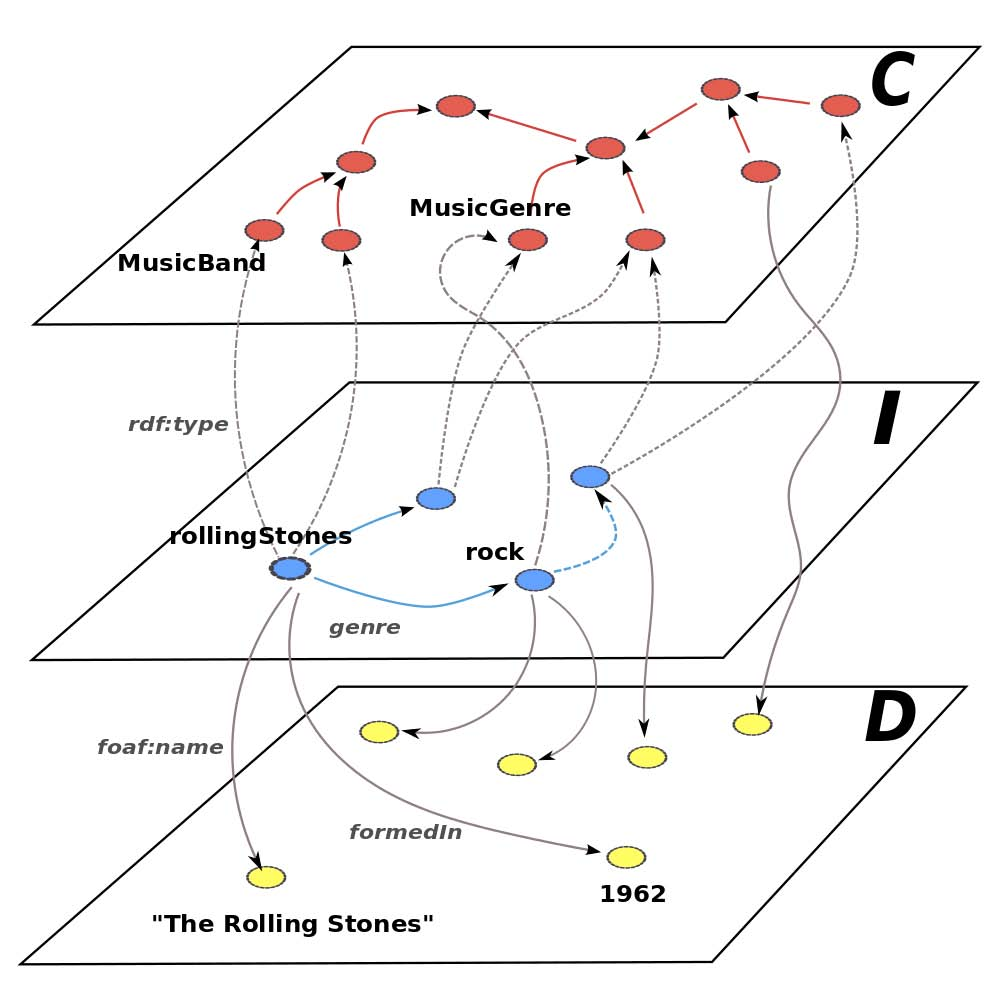
\includegraphics[height=.8\textheight]{instances.png}}
  {\tiny From Harispe et al., Semantic Similarity From Natural
    Language And Ontology Analysis, 2015.}
\end{frame}

\begin{frame}
  \frametitle{How to measure similarity?}
  \begin{itemize}
  \item Shortest Path
    \begin{itemize}
    \item applicable to arbitrary knowledge graphs
    \item does not capture similarity well over all edge types, e.g.,
      {\em disjointWith}, {\em differentFrom}, {\em opposite-of}, etc.
    \end{itemize}
  \item Random Walk
    \begin{itemize}
    \item with or without restart
    \item iterated
    \item does not consider edge labels $\Rightarrow$ captures only
      adjacency of nodes
    \item scores whole graph with {\em probability} of being in a
      state
    \item can take multiple seed nodes
      \begin{itemize}
      \item widely used to find disease genes
      \end{itemize}
    \end{itemize}
  \end{itemize}
\end{frame}

\begin{frame}
  \frametitle{How to measure similarity?}
  \begin{itemize}
  \item feature learning on knowledge graph
    \pause
  \item e.g., iterated, edge-labeled random walk
    \begin{itemize}
%    \item over instances and classes
    \item walks form {\em sentences}
    \item sentences form a {\em corpus}
    \item feature learning on corpus through Word2Vec (or factorization
      of co-occurrence matrix)
    % \item RDF2Vec:
    %   \url{http://data.dws.informatik.uni-mannheim.de/rdf2vec/}
      \pause
    \item with support for reasoning over bio-ontologies:
        \url{https://github.com/bio-ontology-research-group/walking-rdf-and-owl}
        % \begin{itemize}
        % \item (self-promotion warning)
        % \end{itemize}
      \item Onto2Vec: \url{https://github.com/bio-ontology-research-group/onto2vec/}
    \end{itemize}
    \pause
  \item Translational knowledge graph embeddings: TransE, TransR, TransE, HolE, etc.
    \begin{itemize}
    \item analogy-based
    \item \url{https://github.com/thunlp/KB2E}
    \end{itemize}
    \pause
  \item generates (dense) feature vectors for nodes (classes,
    instances) and relations
  \end{itemize}
\end{frame}

\section{Machine learning and ontologies}

\begin{frame}
  \frametitle{Knowledge graph embeddings}
  \begin{definition}
    Let $KG = (V, E, L; \vdash)$ be a knowledge graph with a set of
    vertices $V$, a set of edges $E \subseteq V \times V$, a label
    function $L: V \cup E \mapsto Lab$ that assigns labels from a
    label set $Lab$ to vertices and edges, and an inference relation
    $\vdash$. A knowledge graph embedding is a function
    $f_\eta : KG \mapsto \mathbf{R}^n$ (subject to certain
    constraints).
  \end{definition}
\end{frame}

\begin{frame}
  \frametitle{Neuro-symbolic feature learning}
  \begin{columns}
    \begin{column}{.6\textwidth}
      \resizebox{1\textwidth}{!}{%
        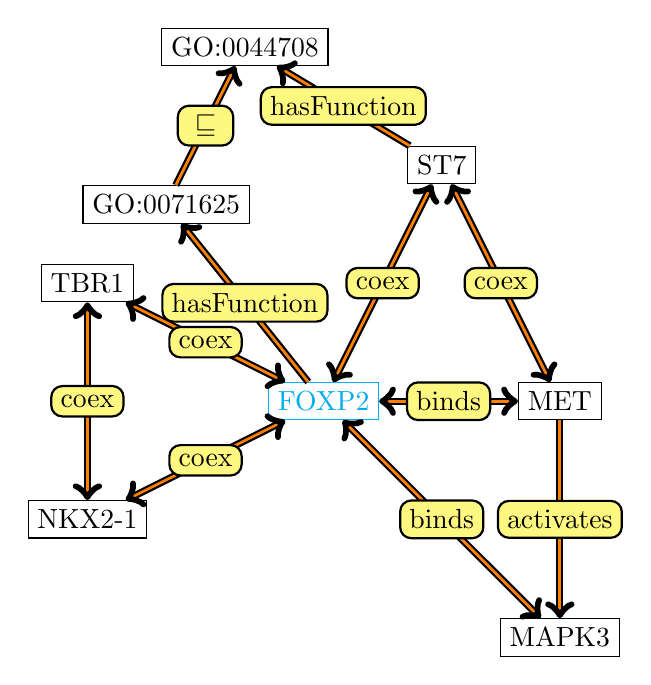
\begin{tikzpicture}
%          \SetUpEdge[lw = 1pt, color = black]
          \GraphInit[vstyle=Shade]
          \tikzset{
            LabelStyle/.style = { rectangle, rounded corners, draw,
              minimum width = 2em, fill = yellow!50,
              text = black },
            VertexStyle/.append style = { inner sep=5pt,
              font = \Large\bfseries},
            EdgeStyle/.append style = {->} }
          
          \SetGraphUnit{5}
          % \tikzset{VertexStyle/.append style={fill}}
          % \tikzset{EdgeStyle/.style={->}}
          \node[draw, color=cyan] (FOXP2) at (0,0) {FOXP2};
          \node[draw] (MET) at (3,0) {MET};
          \node[draw] (ST7) at (1.5,3) {ST7};
          \node[draw] (MAPK3) at (3,-3) {MAPK3};
          \node[draw] (GO0071625) at (-2,2.5) {GO:0071625};
          \node[draw] (GO0044708) at (-1,4.5) {GO:0044708};
          \node[draw] (TBR1) at (-3,1.5) {TBR1};
          \node[draw] (NKX2-1) at (-3,-1.5) {NKX2-1};
          \begin{scope}[/tikz/handle active characters in nodes=false]
          \Edge[label=activates](MET)(MAPK3)
          \Edge[label=hasFunction](FOXP2)(GO0071625)
          \Edge[label=hasFunction](ST7)(GO0044708)
          \Edge[label=$\sqsubseteq$](GO0071625)(GO0044708)

          \tikzset{EdgeStyle/.append style={<->}}
          \Edge[label=binds](FOXP2)(MET)
          \Edge[label=binds](FOXP2)(MAPK3)
          \Edge[label=coex](FOXP2)(TBR1)
          \Edge[label=coex](FOXP2)(NKX2-1)
          \Edge[label=coex](FOXP2)(ST7)
          \Edge[label=coex](MET)(ST7)
          \Edge[label=coex](NKX2-1)(TBR1)
          \end{scope}
          % \tikzset{EdgeStyle/.style={->}}
          % \Edge[label=hf](FOXP2)(GO0044708)
          % \draw[label=binds] (FOXP2) to (MET);
          % \Edge[label=binds](FOXP2)(MET)
          % \Edge[label=activates](MET)(MAPK3)
          % \Edge[label=coexpressed-with](FOXP2)(FOXP4)
          
        \end{tikzpicture}
      }
    \end{column}
    \begin{column}{.4\textwidth}
      \begin{itemize}
      \item task: predict if FOXP2 is involved in disease $D$
      \item task: what chemicals could (directly or indirectly) affect
        FOXP2's function?
      \item which features are relevant?
      \end{itemize}
    \end{column}
  \end{columns}
      
\end{frame}

\begin{frame}
  \frametitle{Neuro-symbolic feature learning}
  \begin{columns}
    \begin{column}{.6\textwidth}
      \resizebox{1\textwidth}{!}{%
        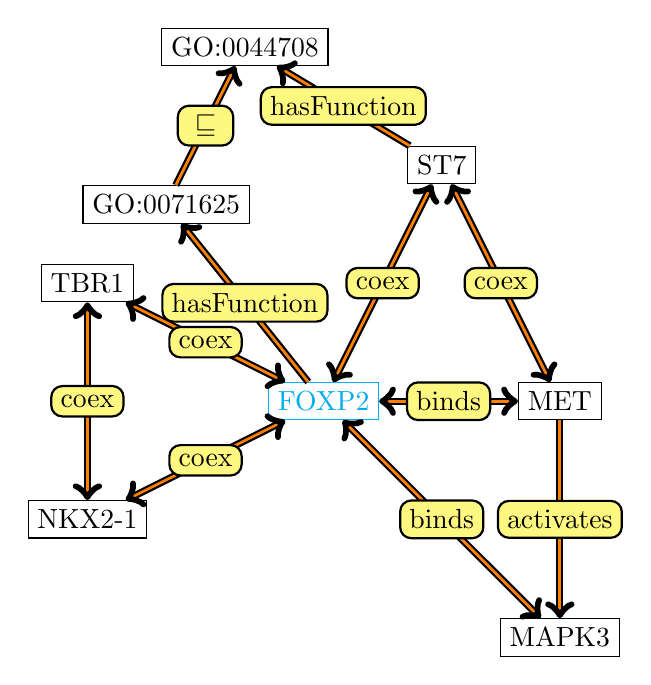
\begin{tikzpicture}
%          \SetUpEdge[lw = 1pt, color = black]
          \GraphInit[vstyle=Shade]
          \tikzset{
            LabelStyle/.style = { rectangle, rounded corners, draw,
              minimum width = 2em, fill = yellow!50,
              text = black },
            VertexStyle/.append style = { inner sep=5pt,
              font = \Large\bfseries},
            EdgeStyle/.append style = {->} }
          
          \SetGraphUnit{5}
          % \tikzset{VertexStyle/.append style={fill}}
          % \tikzset{EdgeStyle/.style={->}}
          \node[draw, color=cyan] (FOXP2) at (0,0) {FOXP2};
          \node[draw] (MET) at (3,0) {MET};
          \node[draw] (ST7) at (1.5,3) {ST7};
          \node[draw] (MAPK3) at (3,-3) {MAPK3};
          \node[draw] (GO0071625) at (-2,2.5) {GO:0071625};
          \node[draw] (GO0044708) at (-1,4.5) {GO:0044708};
          \node[draw] (TBR1) at (-3,1.5) {TBR1};
          \node[draw] (NKX2-1) at (-3,-1.5) {NKX2-1};
          \begin{scope}[/tikz/handle active characters in nodes=false]
          \Edge[label=activates](MET)(MAPK3)
          \Edge[label=hasFunction](FOXP2)(GO0071625)
          \Edge[label=hasFunction](ST7)(GO0044708)
          \Edge[label=$\sqsubseteq$](GO0071625)(GO0044708)

          \tikzset{EdgeStyle/.append style={<->}}
          \Edge[label=binds](FOXP2)(MET)
          \Edge[label=binds](FOXP2)(MAPK3)
          \Edge[label=coex](FOXP2)(TBR1)
          \Edge[label=coex](FOXP2)(NKX2-1)
          \Edge[label=coex](FOXP2)(ST7)
          \Edge[label=coex](MET)(ST7)
          \Edge[label=coex](NKX2-1)(TBR1)
          \end{scope}
          % \tikzset{EdgeStyle/.style={->}}
          % \Edge[label=hf](FOXP2)(GO0044708)
          % \draw[label=binds] (FOXP2) to (MET);
          % \Edge[label=binds](FOXP2)(MET)
          % \Edge[label=activates](MET)(MAPK3)
          % \Edge[label=coexpressed-with](FOXP2)(FOXP4)
          
        \end{tikzpicture}
      }
    \end{column}
    \begin{column}{.4\textwidth}
      % \begin{itemize}
      % \item task: predict if FOXP2 is involved in disease $D$
      % \item which features are relevant?
      %   \pause
      % \item learn relevant features $\Rightarrow$ knowledge graph
      %   embedding
      %   \pause
      % \item incorporate inferences by deductively closing the graph
      % \end{itemize}
    \end{column}
  \end{columns}
      
\end{frame}

\begin{frame}
  \frametitle{Neuro-symbolic feature learning}
  \begin{columns}
    \begin{column}{.6\textwidth}
      \resizebox{1\textwidth}{!}{%
        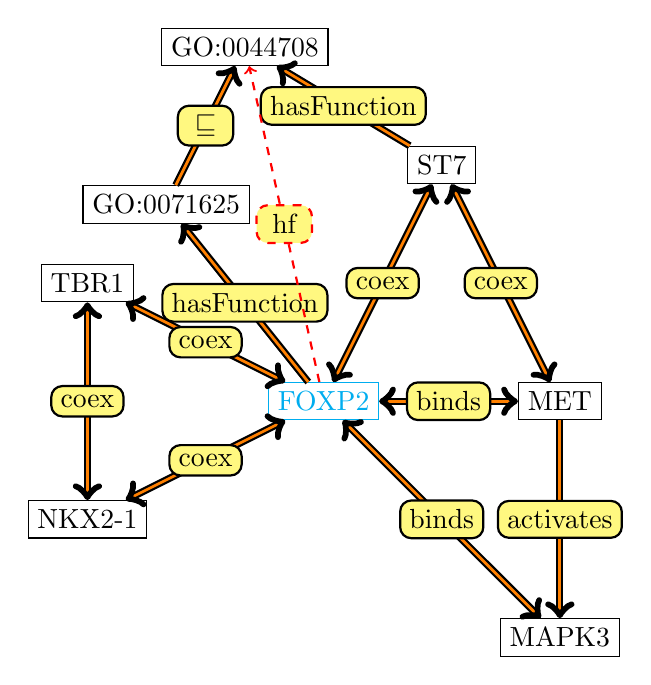
\begin{tikzpicture}
%          \SetUpEdge[lw = 1pt, color = black]
          \GraphInit[vstyle=Shade]
          \tikzset{
            LabelStyle/.style = { rectangle, rounded corners, draw,
              minimum width = 2em, fill = yellow!50,
              text = black },
            VertexStyle/.append style = { inner sep=5pt,
              font = \Large\bfseries},
            EdgeStyle/.append style = {->} }
          
          \SetGraphUnit{5}
          % \tikzset{VertexStyle/.append style={fill}}
          % \tikzset{EdgeStyle/.style={->}}
          \node[draw, color=cyan] (FOXP2) at (0,0) {FOXP2};
          \node[draw] (MET) at (3,0) {MET};
          \node[draw] (ST7) at (1.5,3) {ST7};
          \node[draw] (MAPK3) at (3,-3) {MAPK3};
          \node[draw] (GO0071625) at (-2,2.5) {GO:0071625};
          \node[draw] (GO0044708) at (-1,4.5) {GO:0044708};
          \node[draw] (TBR1) at (-3,1.5) {TBR1};
          \node[draw] (NKX2-1) at (-3,-1.5) {NKX2-1};
          \begin{scope}[/tikz/handle active characters in nodes=false]
          \Edge[label=activates](MET)(MAPK3)
          \Edge[label=hasFunction](FOXP2)(GO0071625)
          \Edge[label=hasFunction](ST7)(GO0044708)
          \Edge[label=$\sqsubseteq$](GO0071625)(GO0044708)

          \tikzset{EdgeStyle/.append style={<->}}
          \Edge[label=binds](FOXP2)(MET)
          \Edge[label=binds](FOXP2)(MAPK3)
          \Edge[label=coex](FOXP2)(TBR1)
          \Edge[label=coex](FOXP2)(NKX2-1)
          \Edge[label=coex](FOXP2)(ST7)
          \Edge[label=coex](MET)(ST7)
          \Edge[label=coex](NKX2-1)(TBR1)

          \tikzset{EdgeStyle/.style={->}}
          \Edge[label=hf, color=red, style=dashed](FOXP2)(GO0044708)
          \end{scope}
          % \draw[label=binds] (FOXP2) to (MET);
          % \Edge[label=binds](FOXP2)(MET)
          % \Edge[label=activates](MET)(MAPK3)
          % \Edge[label=coexpressed-with](FOXP2)(FOXP4)
          
        \end{tikzpicture}
      }
    \end{column}
    \begin{column}{.4\textwidth}
      \begin{itemize}
        \pause
      \item :FOXP2 :binds :MET :coex :ST7 :hasFunction GO:0044708
        \pause
      \item :FOXP2 :hasFunction GO:0071625 subClassOf GO:0044708
        \pause
      \item :FOXP2 :coex :TBR1 :coex :NKX2-1 :coex :TBR1 :coex ...
      \end{itemize}
    \end{column}
  \end{columns}
\end{frame}

\begin{frame}
  \frametitle{Neuro-symbolic feature learning}
  \begin{itemize}
  % \item iterated random walk from each node (in a knowledge graph
  %   consisting of instances and classes) defines sentences
  % \item one embedding for every node and edge type in our graph
  \item skip-gram model learns representation/features for each node
    \begin{itemize}
    \item Word2Vec model, given a word predicts context
    \item use local and non-local information
    \end{itemize}
  \item automated reasoning deductively closes the knowledge graph
    \begin{itemize}
    \item making this a neuro-symbolic model
    \end{itemize}
  \item useful for edge prediction, similarity, clustering, as feature
    vectors
    \begin{itemize}
    \item edge prediction: analogy, classifier (e.g., SVM)
    \end{itemize}
  \end{itemize}
\end{frame}

\begin{frame}
  \frametitle{Neuro-symbolic feature learning}
  \centerline{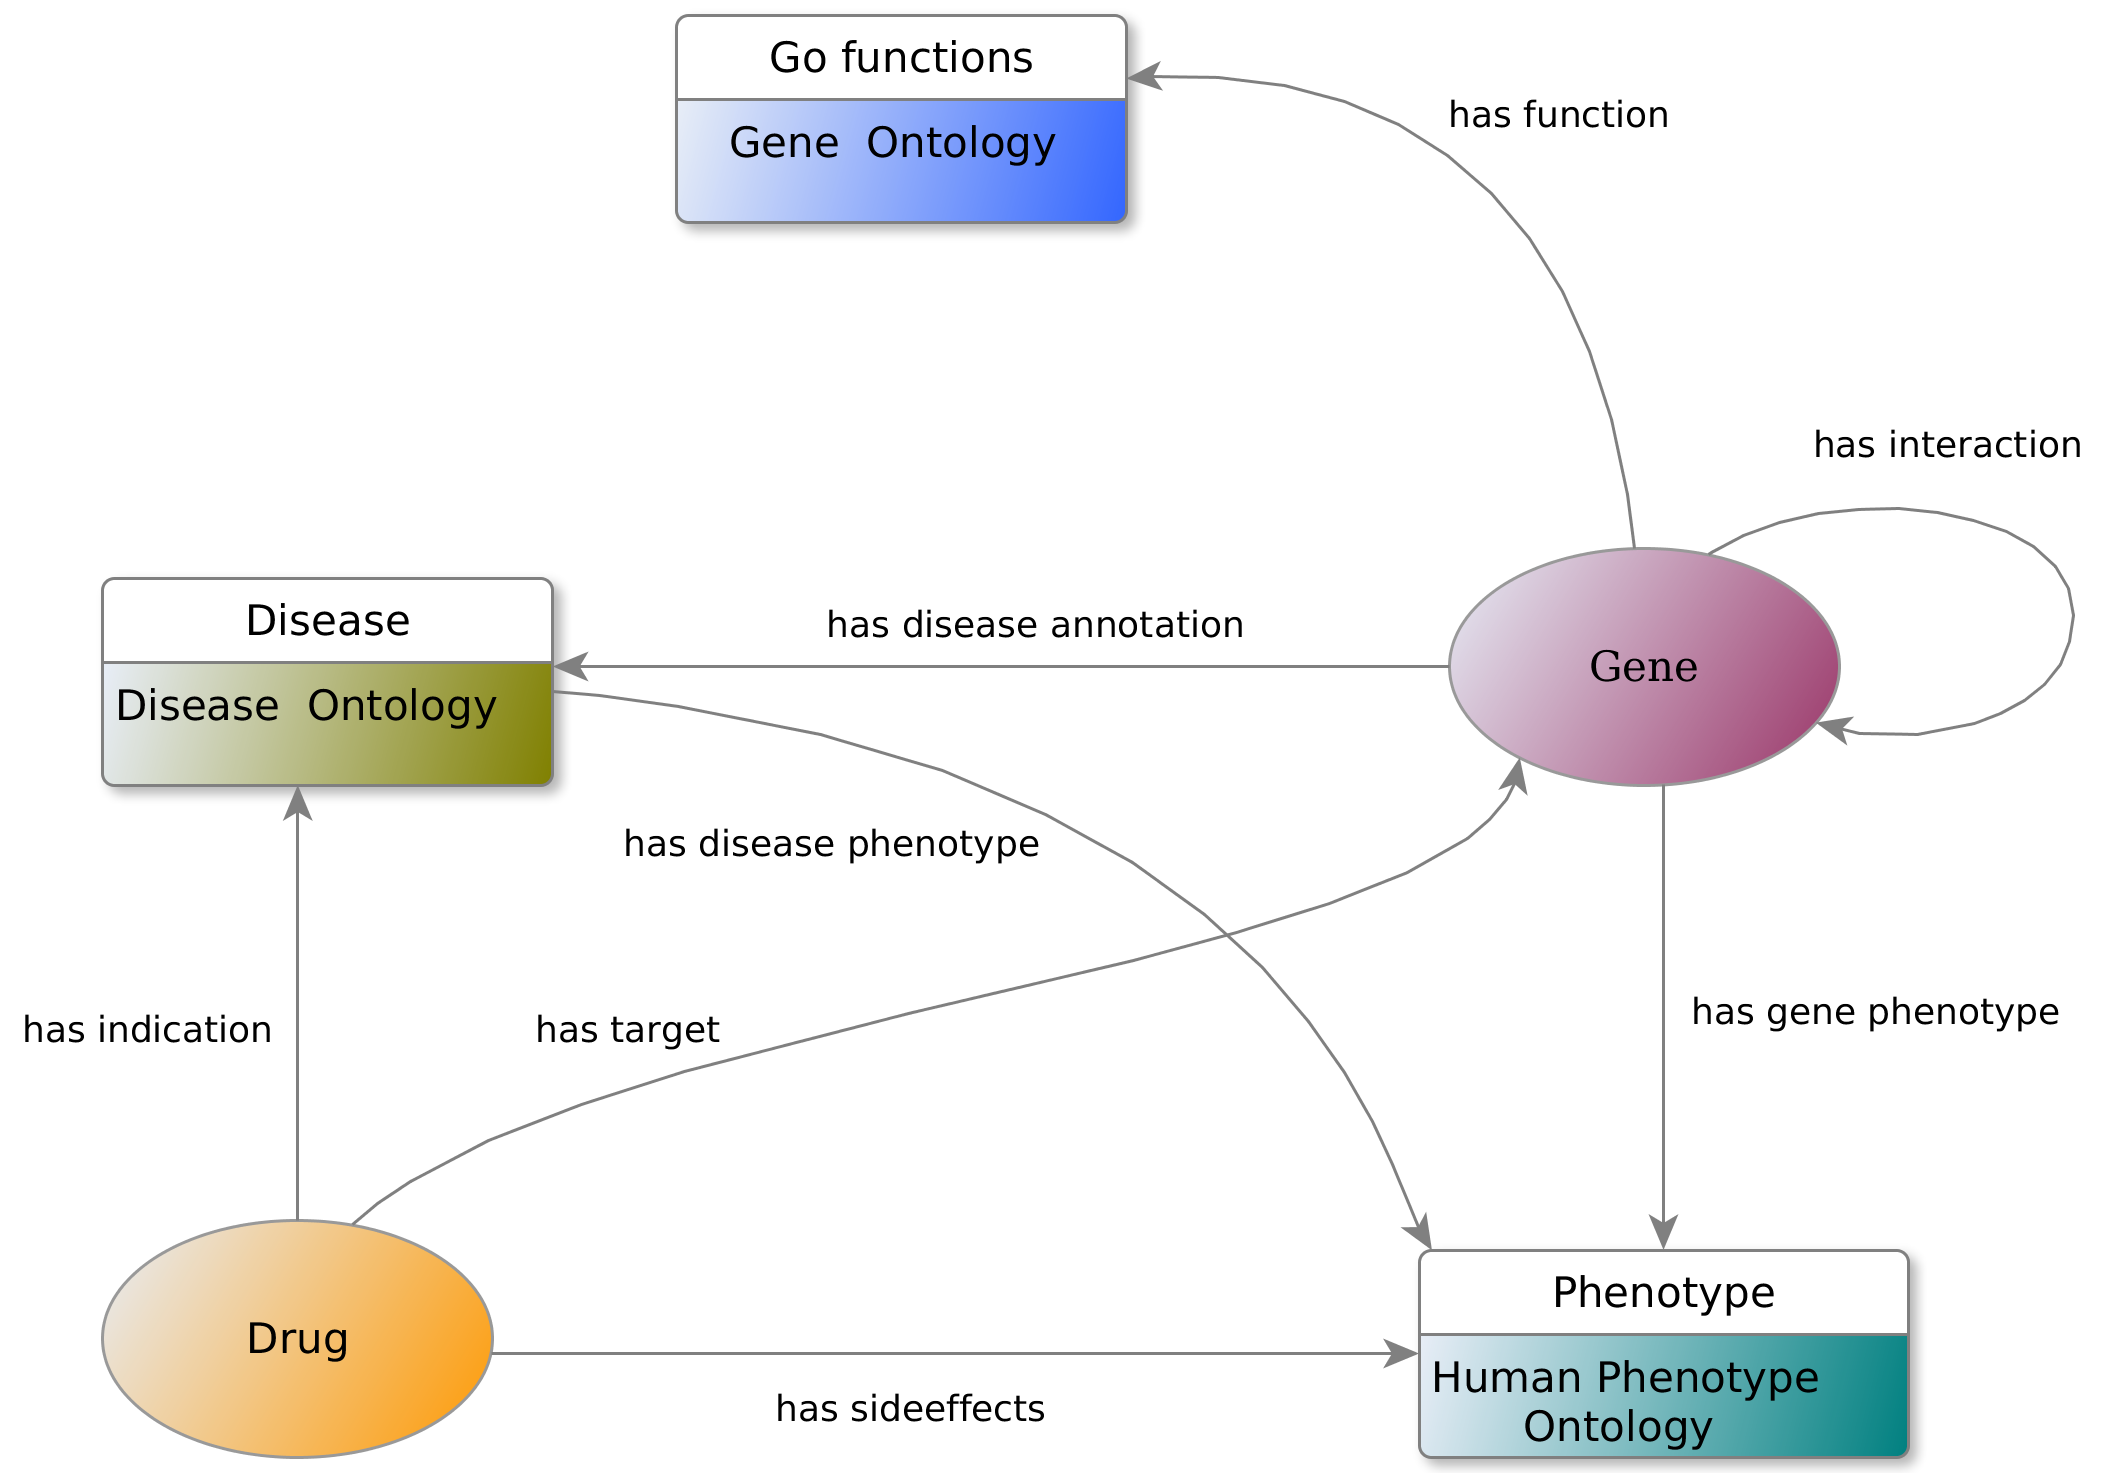
\includegraphics[width=\textwidth]{rdf-walking-datasets.png}}
\end{frame}

\begin{frame}
  \frametitle{Neuro-symbolic feature learning}
    \begin{table}[ht!]
  \resizebox{\textwidth}{!}{%
      \centering
      \begin{tabular}{@{}lllcccc@{}}\toprule 
        \multirow{2}{*}{Object property} 
        & Source type & Target type &\multicolumn{2}{c}{Without reasoning}&\multicolumn{2}{c}{With reasoning}\\
        &&& F-measure & AUC & F-measure & AUC \\
        \midrule
        has target & Drug & Gene/Protein & 0.94 & 0.97 & 0.94 & 0.98 \\
        has disease annotation & Gene/Protein & Disease & 0.89 & 0.95 & 0.89 & 0.95 \\
        has side-effect$^*$ & Drug & Phenotype & 0.86 & 0.93 & 0.87 & 0.94 \\
        has interaction & Gene/Protein & Gene/Protein & 0.82 & 0.88 & 0.82 & 0.88\\
        has function$^*$ & Gene/Protein & Function & 0.85 & 0.95 & 0.83 & 0.91 \\
        has gene phenotype$^*$  & Gene/Protein & Phenotype & 0.84 & 0.91 & 0.82 & 0.90  \\
        has indication & Drug & Disease & 0.72 & 0.79 & 0.76 & 0.83 \\
        has disease phenotype$^*$  & Disease & Phenotype & 0.72 & 0.78 & 0.70 & 0.77 \\
      \end{tabular}
  }
\end{table}
\vfill
{\tiny Alsharani et al. Neuro-symbolic representation learning on
biological knowledge graphs. Bioinformatics, 2017.}
\end{frame}

\begin{frame}
  \frametitle{Multi-modal feature learning}
    \begin{quote}
      The \only<1,2>{\underline{forkhead-box P2 (FOXP2)}}\only<3>{\underline{:FOXP2}} gene polymorphism has been
      reported to be involved in the susceptibility to schizophrenia;
      however, few studies have investigated the association between
      \only<1,2>{\underline{FOXP2}}\only<3>{\underline{:FOXP2}} gene polymorphism and clinical symptoms in schizophrenia.
    \end{quote}
  \pause
  \begin{itemize}
  \item \underline{:FOXP2} :binds :MET :coex :ST7 :hasFunction GO:0044708
  \item \underline{:FOXP2} :hasFunction GO:0071625 subClassOf GO:0044708
  \item \underline{:FOXP2} :coex :TBR1 :coex :NKX2-1 :coex :TBR1 :coex ...
  \end{itemize}
\end{frame}

\begin{frame}
  \frametitle{Multi-modal feature learning}
  \centerline{\includegraphics[width=\textwidth]{multimodal_workflow.pdf}}
\end{frame}


\begin{frame}
  \frametitle{Multi-modal feature learning: drug targets and indications}
  \centerline{
    \includegraphics[width=.45\textwidth]{DTI_ANN_all.pdf}
    \includegraphics[width=.45\textwidth]{Ind_ANN_all.pdf}
  }
  \vspace{.5cm}
  {\tiny Alshahrani \& H. Drug repurposing through
    multi-modal learning on knowledge graphs. BioRxiv, 2018.}
\end{frame}

\begin{frame}
  \frametitle{Ontologies: axioms, not graphs!}
    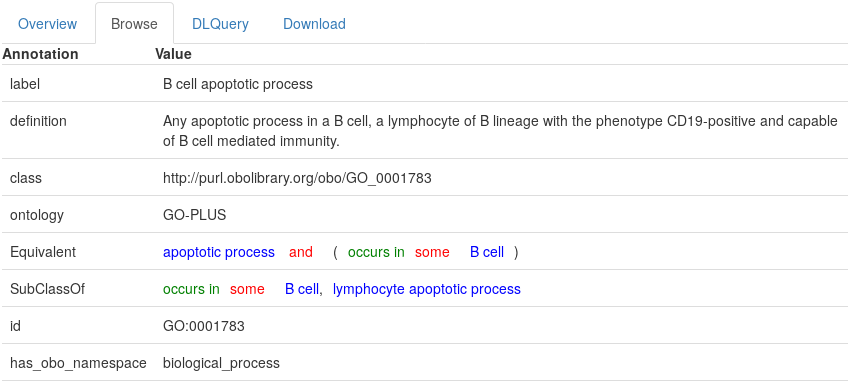
\includegraphics[width=1\textwidth]{bcellapoptosis.png}
\end{frame}

\begin{frame}
  \frametitle{Ontologies: axioms, not graphs!}
  Gene Ontology:
  \begin{itemize}
  \item {\tt behavior DisjointWith: 'developmental process'}
  \item {\tt behavior SubclassOf: only-in-taxon some metazoa}
  \item {\tt 'cell proliferation' DisjointWith: in-taxon some fungi}
  \item {\tt 'cell growth' EquivalentTo: growth and ('results in
      growth of' some cell)}
  \item ...
  \end{itemize}
\end{frame}

% \begin{frame}
%   \frametitle{Ontologies: axioms, not graphs!}
%   \begin{itemize}
%   \item converting ontologies to graphs
%     \begin{itemize}
%     \item loses information
%     \end{itemize}
%   \item relations between ontologies
%   \end{itemize}
% \end{frame}

\begin{frame}
  \frametitle{Ontology embeddings}
  \begin{definition}
    Let $O = (C, R, I; ax; \vdash)$ be an ontology with a set of
    classes $C$, a set of relations $R$, a set of instances $I$, a set
    of axioms $ax$ and an inference relation $\vdash$. An ontology
    embedding is a function $f_\eta : C \cup R \cup I \mapsto
    \mathbf{R}^n$ (subject to certain constraints).
  \end{definition}
  \pause
  We use co-occurrence within $ax^\vdash$ to constrain the embedding
  function, where the constraints on co-occurrence are formulated
  using the Word2Vec skipgram model.
\end{frame}

\begin{frame}
  \frametitle{Onto2Vec}
  \centerline{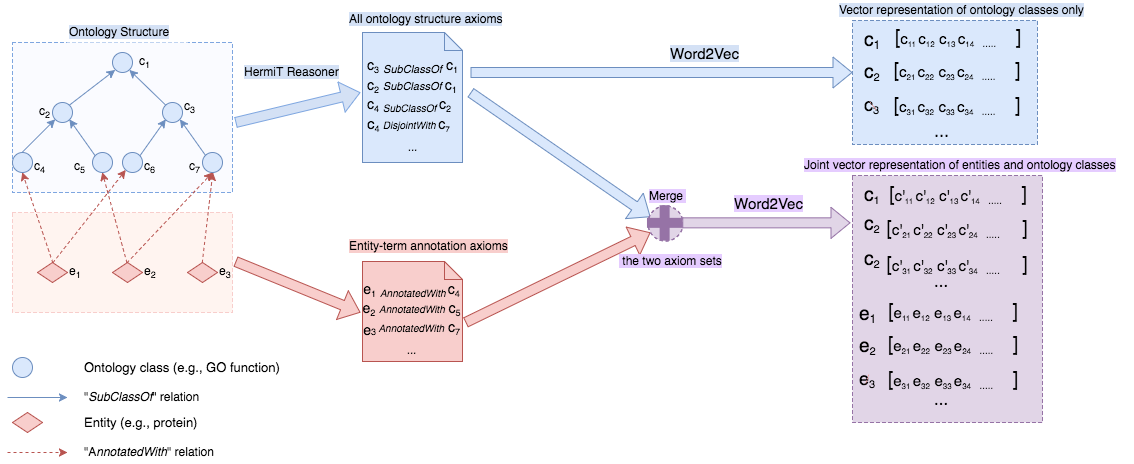
\includegraphics[width=\textwidth]{onto2vecflow.png}}
\end{frame}

\begin{frame}
  \frametitle{Predicting PPIs: trainable similarity measures}
  \centerline{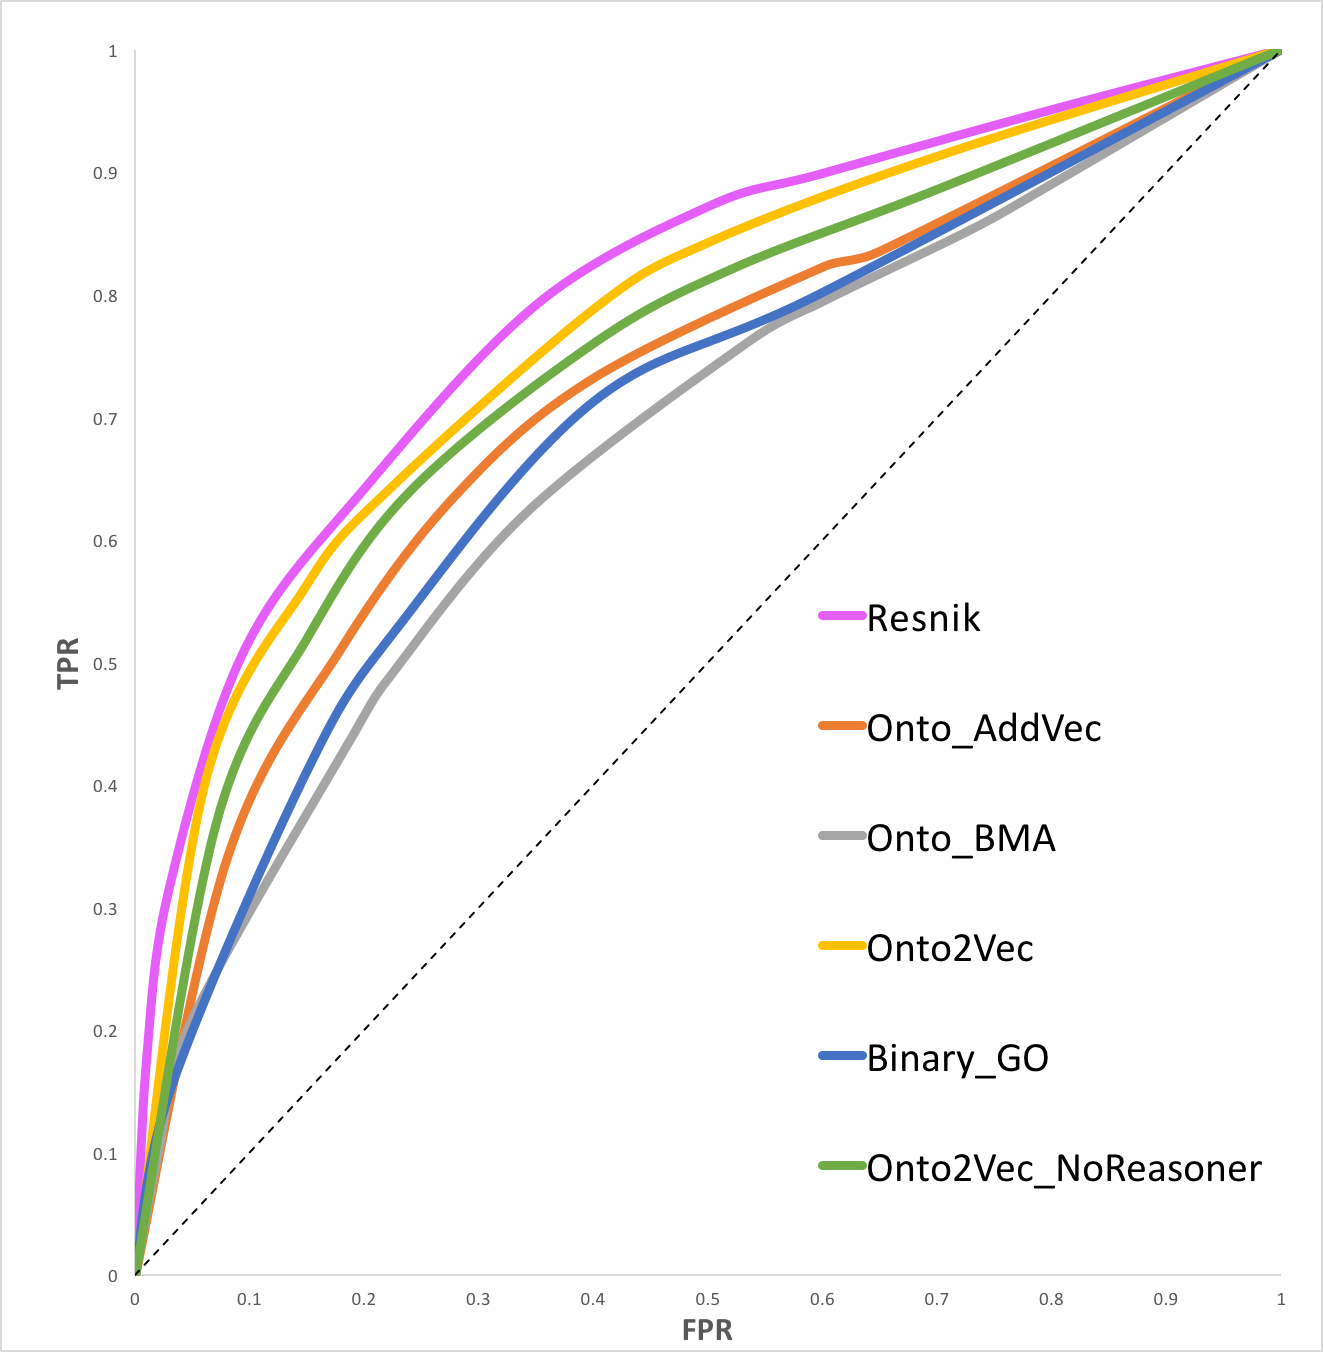
\includegraphics[width=.45\textwidth]{YSTUnsuper1.png}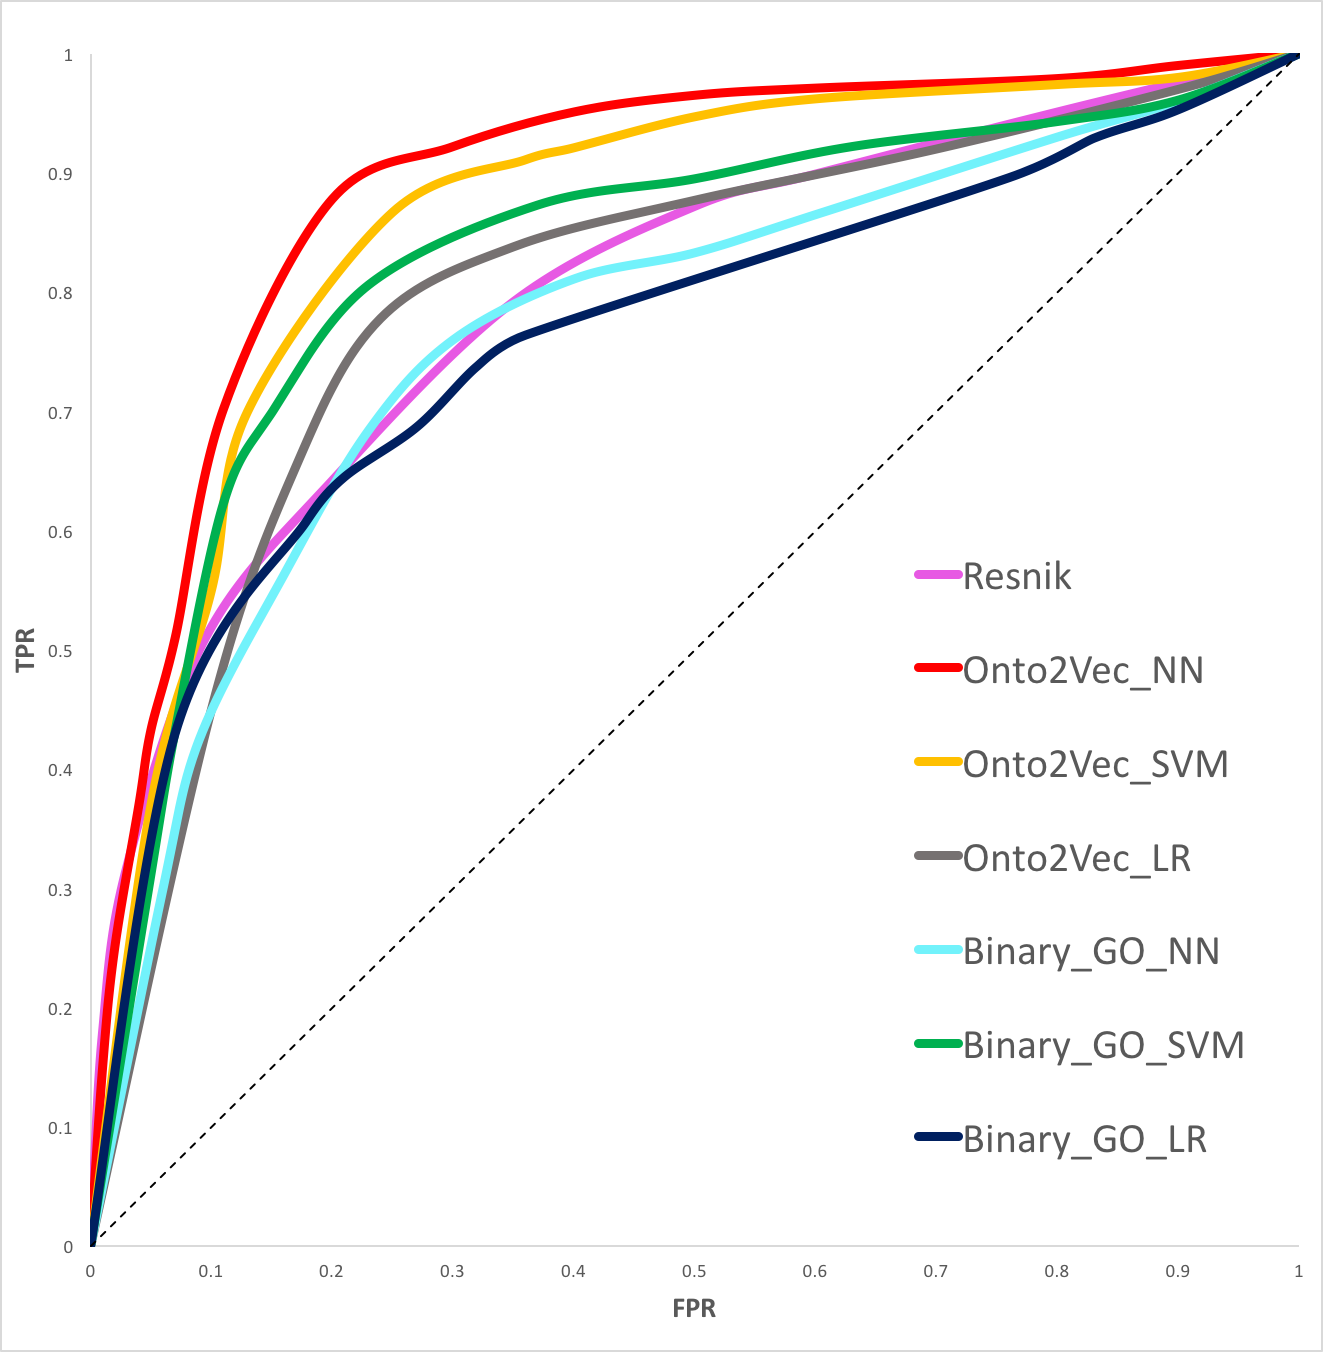
\includegraphics[width=.45\textwidth]{YstUnsup2.png}}
  \vfill
  {\tiny Smaili et al. Onto2Vec: joint vector-based representation of
    biological entities and their ontology-based annotations, Bioinformatics, 2018.}
\end{frame}

\begin{frame}
  \frametitle{Visualizing embeddings}
  \centerline{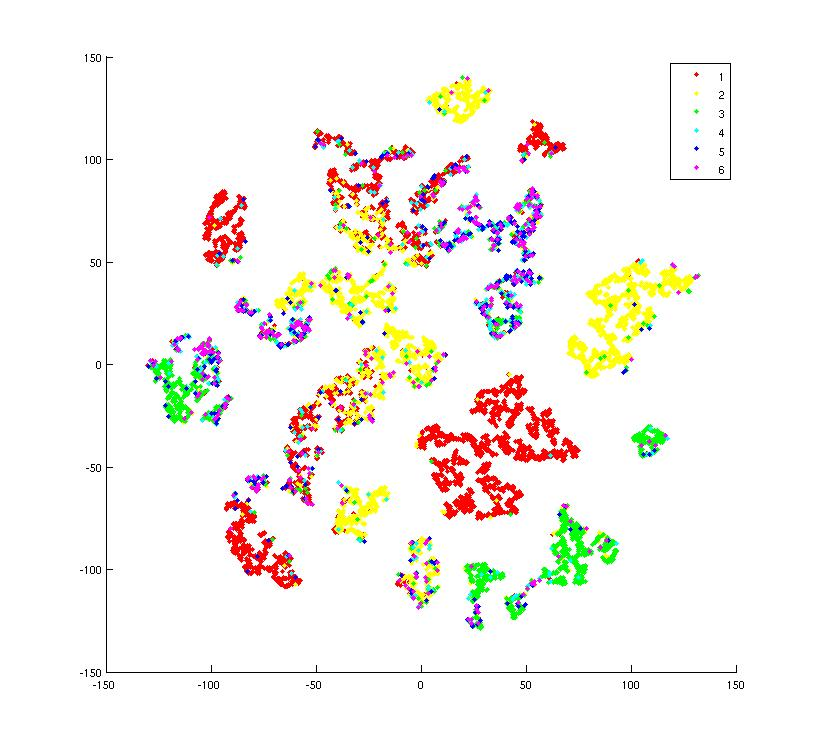
\includegraphics[width=.9\textwidth]{updtsne.jpg}}
\end{frame}

\begin{frame}
  \frametitle{Ontologies Plus Annotations 2 Vec}
  \centerline{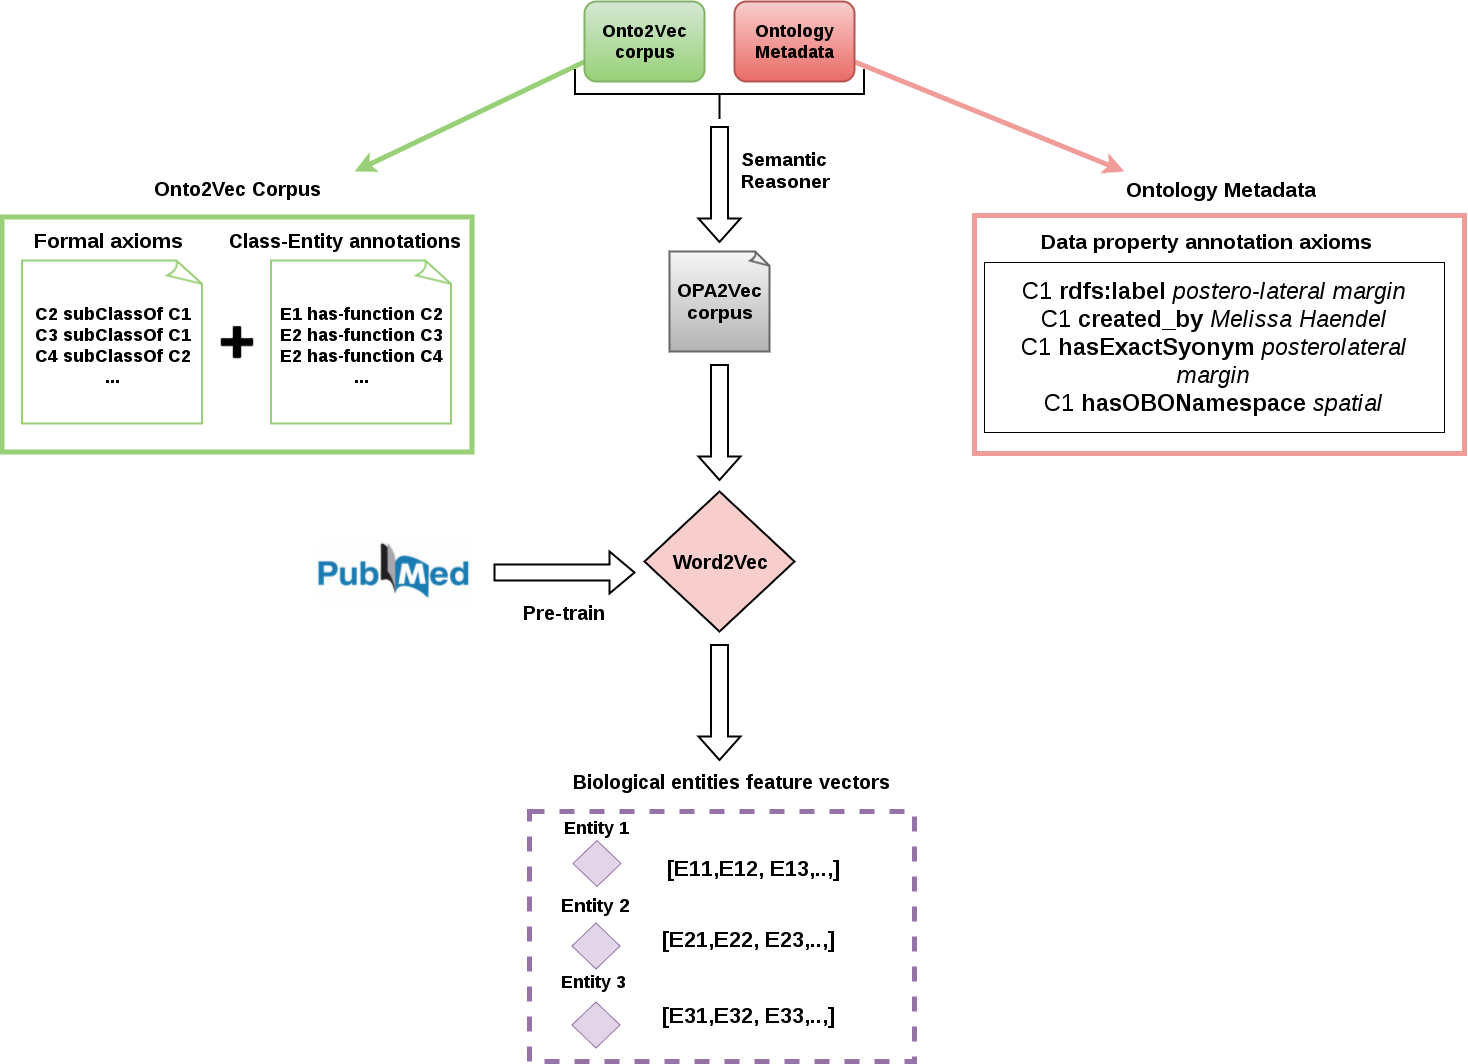
\includegraphics[width=1\textwidth]{opaworkflow16.png}}
\end{frame}

\begin{frame}
  \frametitle{Phenotype-based prediction of candidate genes}
  \centerline{
    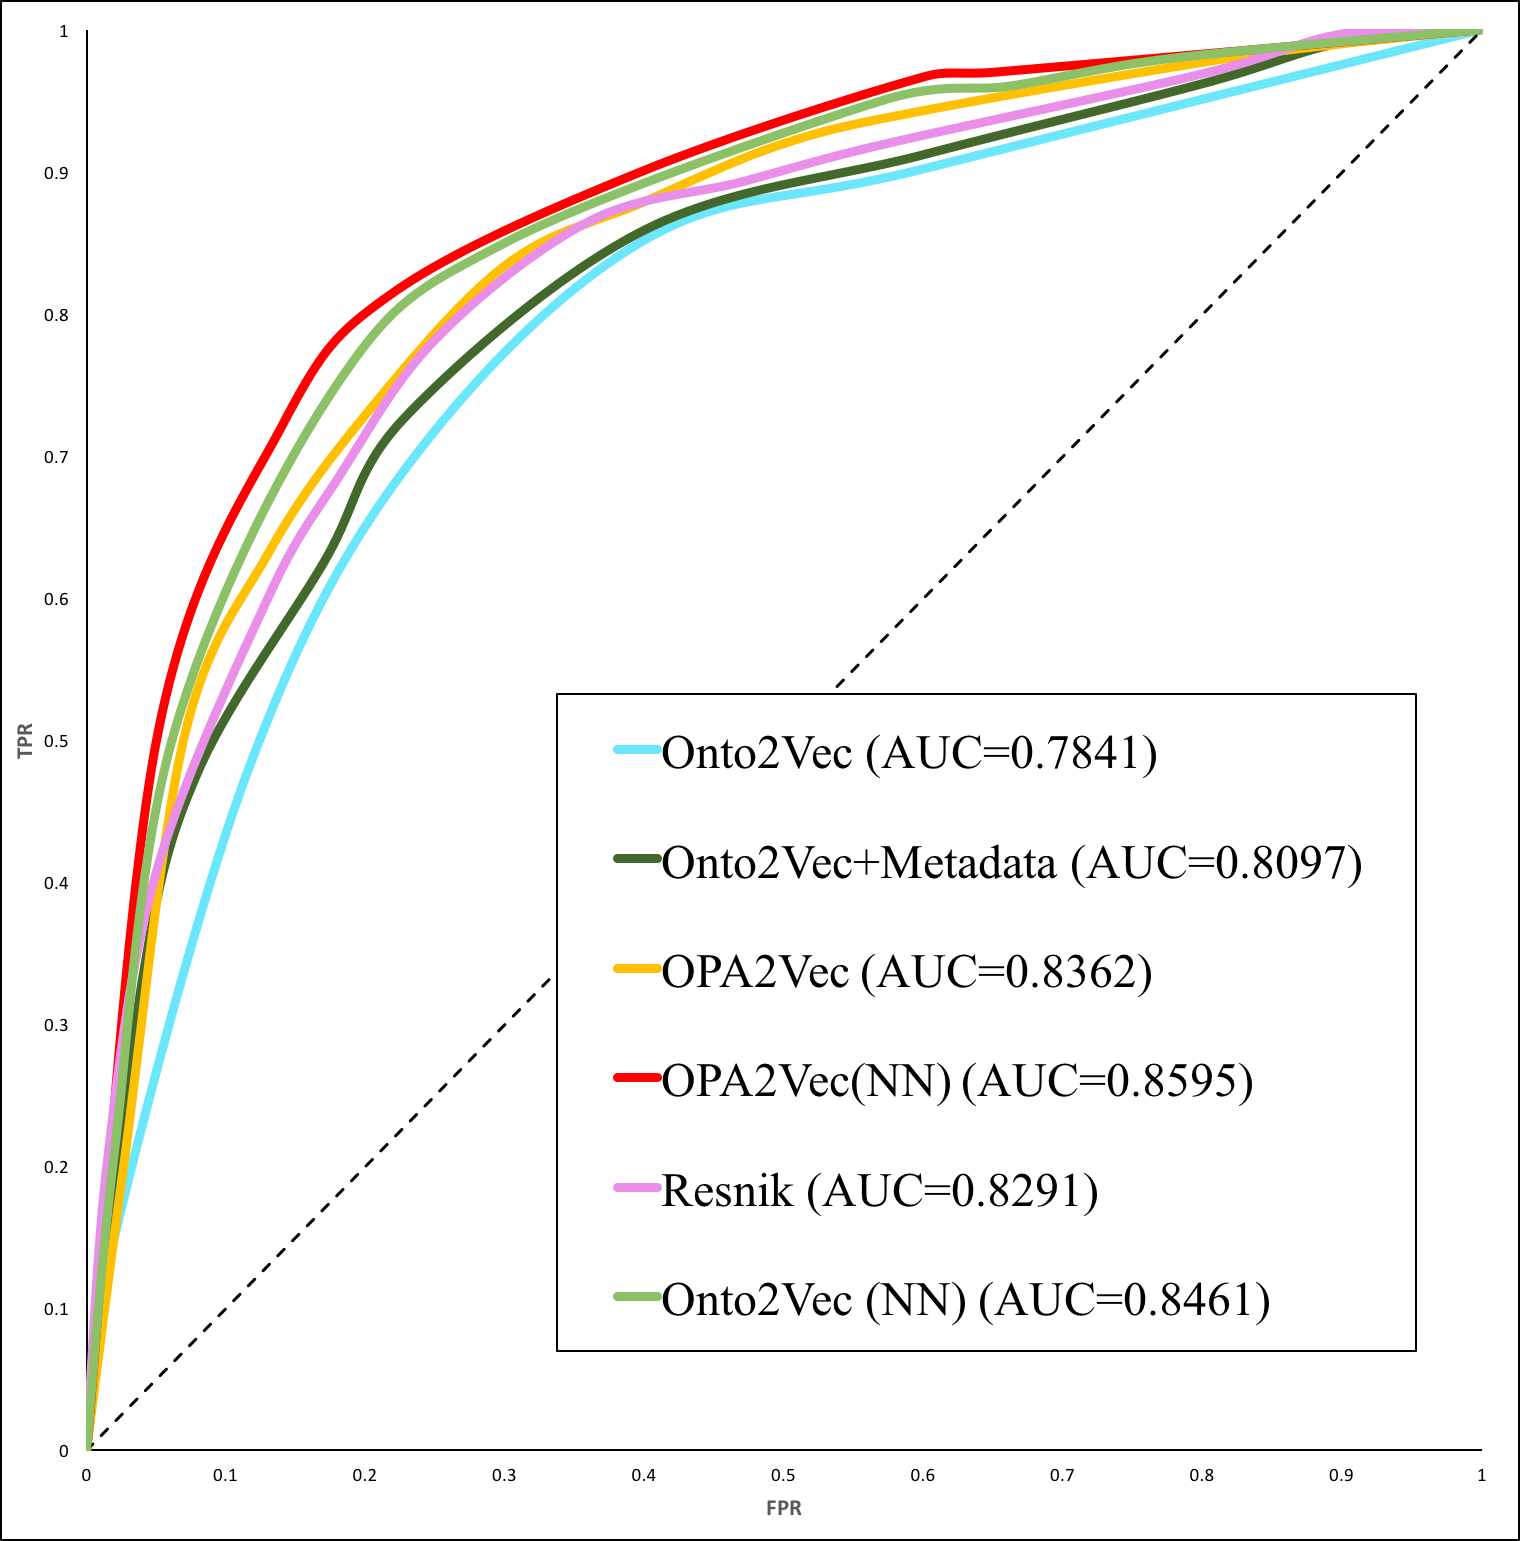
\includegraphics[width=.45\textwidth]{Human_Disease.png}
    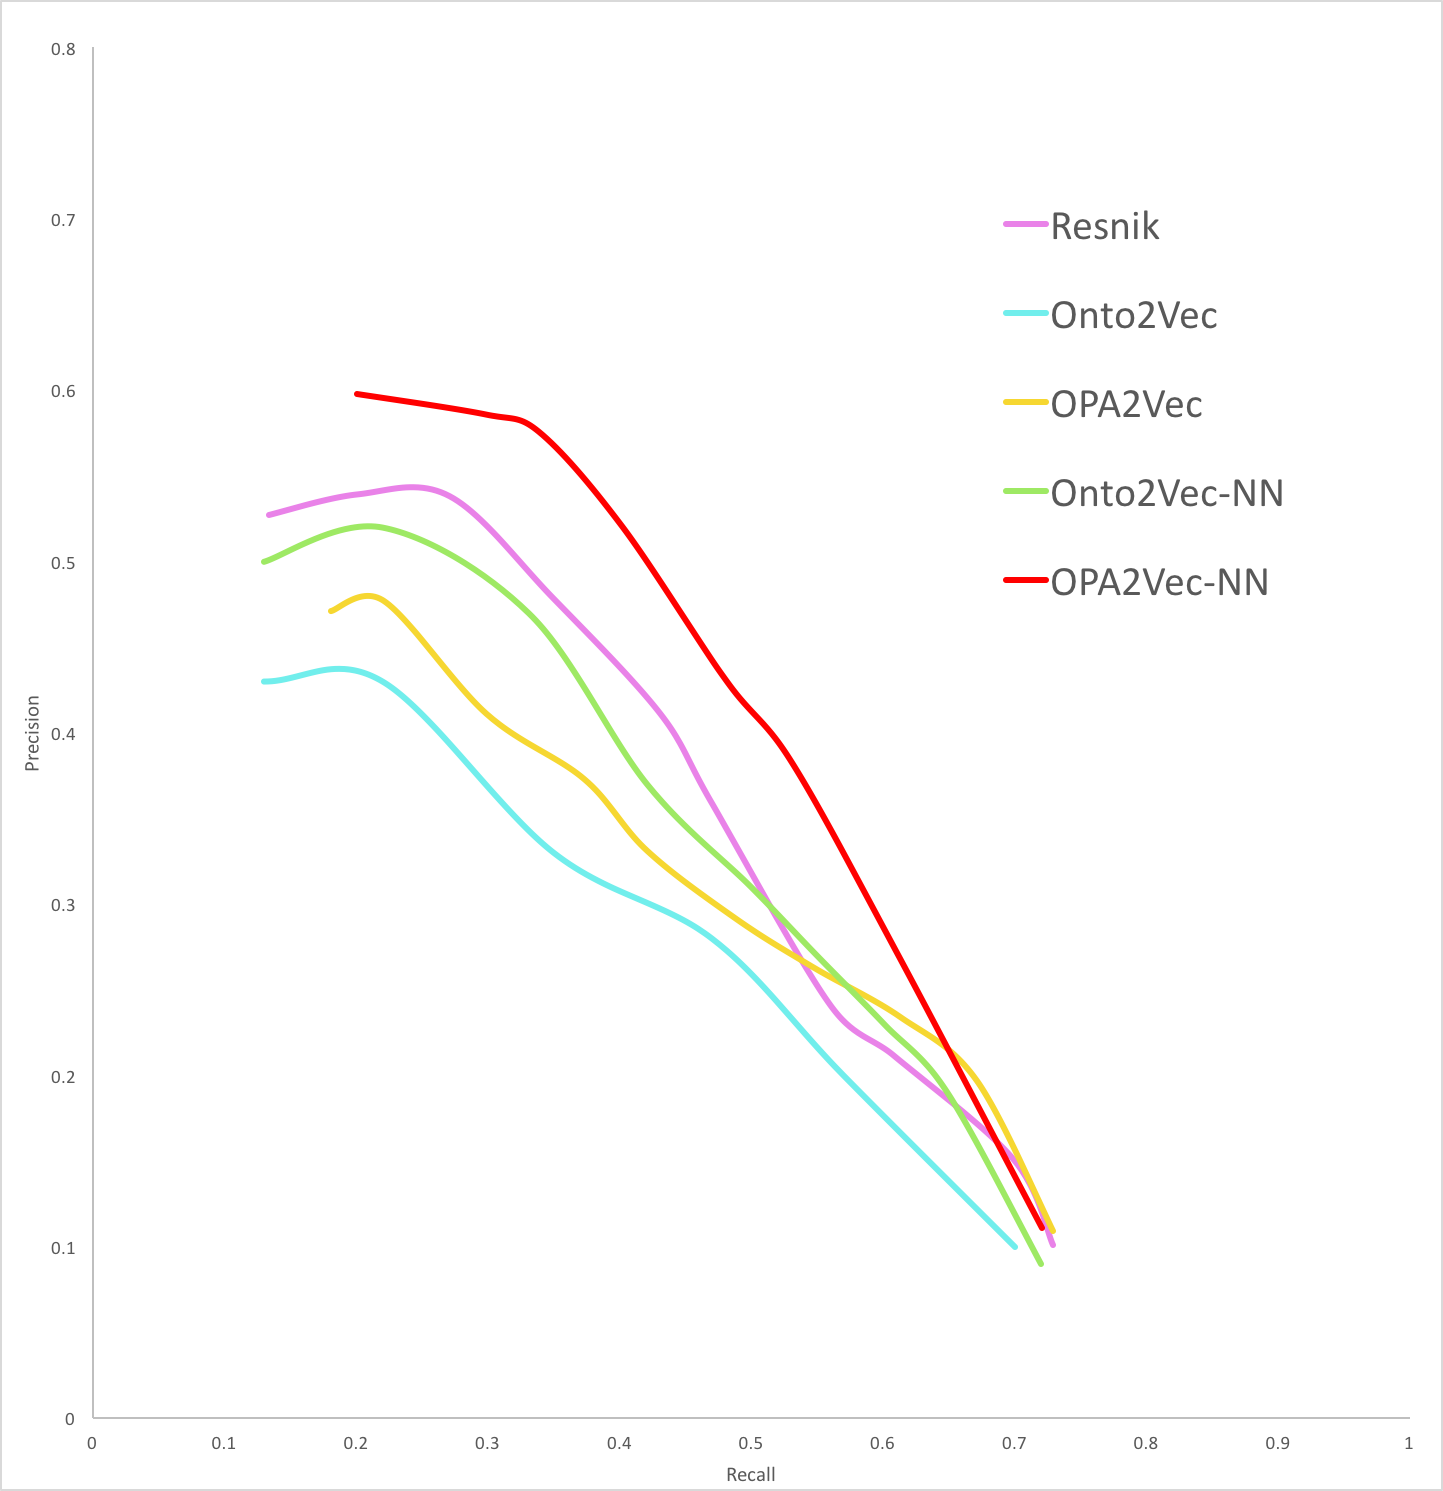
\includegraphics[width=.45\textwidth]{HD.png}
  }
\end{frame}

\begin{frame}
  \frametitle{How to measure similarity?}
  \begin{itemize}
  \item vector-based similarity measure
  \item cosine similarity: $sim(X,Y) = \frac{\sum_{i=1}^n X_i
      Y_i}{\sqrt{\sum_{i=1}^n X_i^2} \sqrt{\sum_{i=1}^n Y_i^2}} $
    \begin{itemize}
    \item bounded between $[-1,1]$
    \end{itemize}
  \item Euclidean distance: $sim(X,Y) = \sqrt{\sum_{i=1}^n (X_i - Y_i)^2}$
    \begin{itemize}
    \item not bounded (and rarely used)
    \end{itemize}
  \item any other kind of function
    \begin{itemize}
    \item Neural Networks can approximate {\em any} function
      (universal approximation theorem)
    \item ``trainable'' semantic similarity measures
    \end{itemize}
  \end{itemize}
\end{frame}

\begin{frame}
  \frametitle{How to measure similarity?}
  \begin{itemize}
  \item many graph based semantic similarity measures for comparing
    two classes
  \item several set-based measures
    \begin{itemize}
    \item directly set-based
    \item merging pair-wise comparison
    \end{itemize}
  \item most useful when comparing instances/annotations
  \item other approaches consider relations between instances:
    \begin{itemize}
    \item path-based
    \item random-walk
    \end{itemize}
  \item very recent: knowledge graph embeddings
    \begin{itemize}
    \item and any vector-based similarity measure
    \end{itemize}
  \end{itemize}
\end{frame}

\begin{frame}
  \frametitle{How to measure similarity?}
  Recommended reading:
  \begin{itemize}
  \item recommended, comprehensive overview: Sebastian Harispe et
    al. Semantic Similarity from Natural Language and Ontology
    Analysis. Morgan \& Claypool Publishers, 2015
  \item Catia Pesquita et al. Semantic Similarity in Biomedical
    Ontologies. PLoS CB, 2009.
  \item Maximilian Nickel et al. A Review of Relational Machine
    Learning for Knowledge Graphs, Proceedings of the IEEE, 2016.
  \end{itemize}
\end{frame}

\begin{frame}
  \frametitle{How to measure similarity: Quiz}
  \begin{itemize}
  \item How many semantic similarity measures are there?
    \begin{enumerate}[a]
    \item One (and it is called The Semantic Similarity Measure)
    \item Three (graph-based, set-based, feature-based)
    \item Many (depending on context, many functions can determine similarity)
    \end{enumerate}
    \pause
  \item Specificity of an ontology class
    \begin{enumerate}[a]
    \item depends on the number of children and ancestors, and the
      depth
    \item depends on the number of instances (or annotations)
    \item can improve similarity estimates significantly
    \end{enumerate}
    \pause
  \item In the presence of (relations between) instances, semantic
    similarity
    \begin{enumerate}[a]
    \item cannot be computed, it only works with ontologies
    \item can be estimated using only class specificity measures
    \item can be computed using knowledge graph embeddings
    \end{enumerate}
  \end{itemize}
\end{frame}

\section{Applications}

\begin{frame}
  \frametitle{Applications of semantic similarity}
  \begin{itemize}
  \item ontologies are used {\em almost everywhere} in biology
  \item many applications of semantic similarity:
    \begin{itemize}
    \item predicting interacting proteins
    \item predict candidate genes
      \begin{itemize}
      \item using the guilt-by-association principle, or without
      \end{itemize}
    \item predict drug targets and indications
    \item as features in machine learning models
    \end{itemize}
  \end{itemize}
\end{frame}

\begin{frame}
  \frametitle{Applications of semantic similarity}
  \begin{block}{Hypothesis}
    Interacting proteins have similar functions.
  \end{block}
  \begin{itemize}
  \item relies on background knowledge about functions (encoded in GO)
  \item ``similarity'' can mean:
    \begin{itemize}
    \item part of the same pathway
    \item siblings of a common super-class
    \item located in the same location
    \end{itemize}
  \item set-based comparison of GO functions
    \begin{itemize}
    \item single GO hierarchy or all?
    \item which similarity measure?
    \end{itemize}
  \end{itemize}
\end{frame}

\begin{frame}
  \frametitle{Applications of semantic similarity}
  \centerline{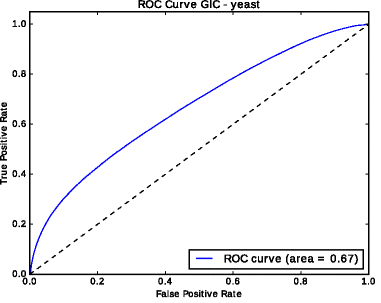
\includegraphics[width=.8\textwidth]{ppi1.png}}
\end{frame}

\begin{frame}
  \frametitle{Applications of semantic similarity}
  \centerline{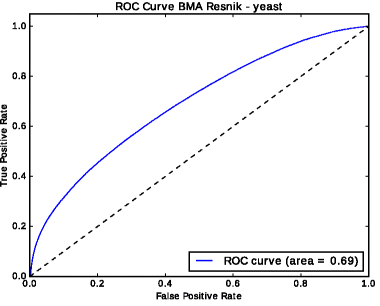
\includegraphics[width=.8\textwidth]{ppi2.png}}
\end{frame}

\begin{frame}
  \frametitle{Applications of semantic similarity}
  \centerline{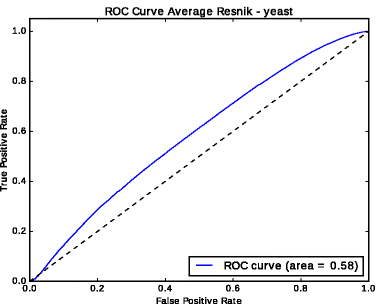
\includegraphics[width=.8\textwidth]{ppi3.png}}
\end{frame}

\begin{frame}
  \frametitle{Applications of semantic similarity}
  \begin{itemize}
  \item no obvious choice of similarity measure
  \item depends on application
    \begin{itemize}
    \item predicting PPIs in different organisms may benefit from a
      different similarity measure!
    \end{itemize}
  \item different similarity measures may react differently to biases
    in data
  \item needs some testing and experience
  \end{itemize}
\end{frame}

\begin{frame}
  \frametitle{Applications of semantic similarity}
  Recommendations:
  \begin{itemize}
  \item use Resnik's information content measure
  \item use Resnik's similarity
  \item use Best Match Average
  \item use the full ontology
  \item classify your ontology using an automated reasoner before
    applying semantic similarity
    \begin{itemize}
    \item although many ontologies come pre-classified
    \end{itemize}
  \item $\Rightarrow$ but there are many exceptions
    \begin{itemize}
    \item similar location $\Rightarrow$ use location subset of GO
    \item developmental phenotypes $\Rightarrow$ use developmental
      branch of phenotype ontology
    \end{itemize}
  \end{itemize}
\end{frame}

\begin{frame}
  \frametitle{Onto2Vec and OPA2Vec}
  Using feature learning to ``learn'' semantic similarity measures in
  a data- and application-driven way...
\end{frame}

\begin{frame}
  \frametitle{Applications of semantic similarity}
  \begin{itemize}
  \item choice of ontology determines the kind of similarity
  \item functional similarity: Gene Ontology
  \item anatomical, structural similarity: anatomy ontologies (Uberon,
    MA, FMA, etc.)
  \item phenotypic similarity: phenotype ontology (HPO, MP, etc.)
  \item chemical structural similarity: ChEBI
  \end{itemize}
\end{frame}

\begin{frame}
  \frametitle{Applications of semantic similarity}
  \begin{itemize}
  \item phenotypic similarity used to:
    \begin{itemize}
    \item diagnosis: similarity between patient phenotypes and disease
      phenotypes
      \begin{itemize}
      \item also between patient phenotypes and gene--phenotype
        associations
      \item Phenomizer: \url{http://compbio.charite.de/phenomizer/}
      \end{itemize}
    \item disease modules: similarity between disease and disease
    \item clustering/stratification: similarity between patient and patient
    \item disease gene discovery: similarity between patient/disease
      phenotypes and gene--phenotype associations
      \begin{itemize}
      \item in humans
      \item in model organisms
      \end{itemize}
    \item drug repurposing: side-effect similarity; similarity between
      side effect profile and gene--disease associations
    \end{itemize}
  \end{itemize}
\end{frame}



\begin{frame}
  \frametitle{Applications of semantic similarity}
  \centerline{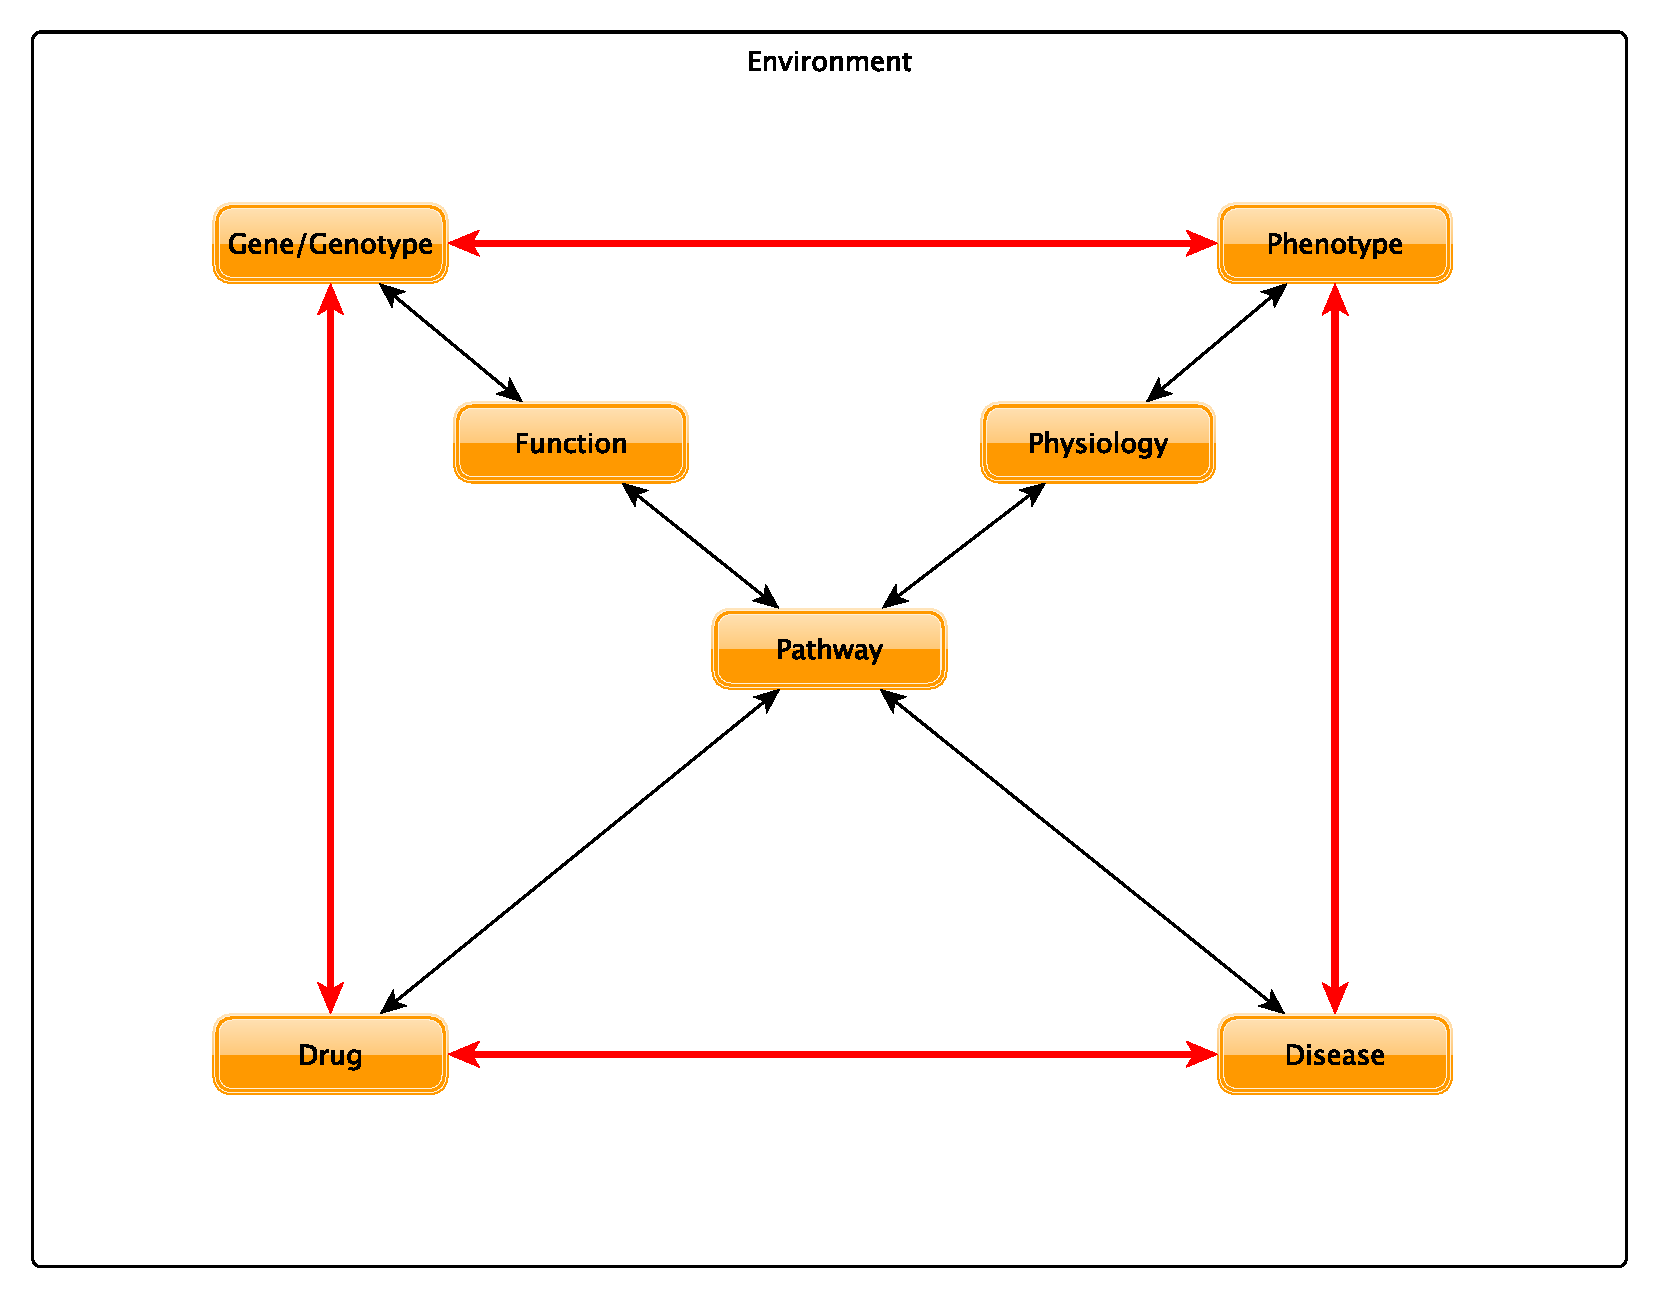
\includegraphics[height=\textheight]{vision1.pdf}}
\end{frame}

\begin{frame}
  \frametitle{Applications of semantic similarity}
  \centerline{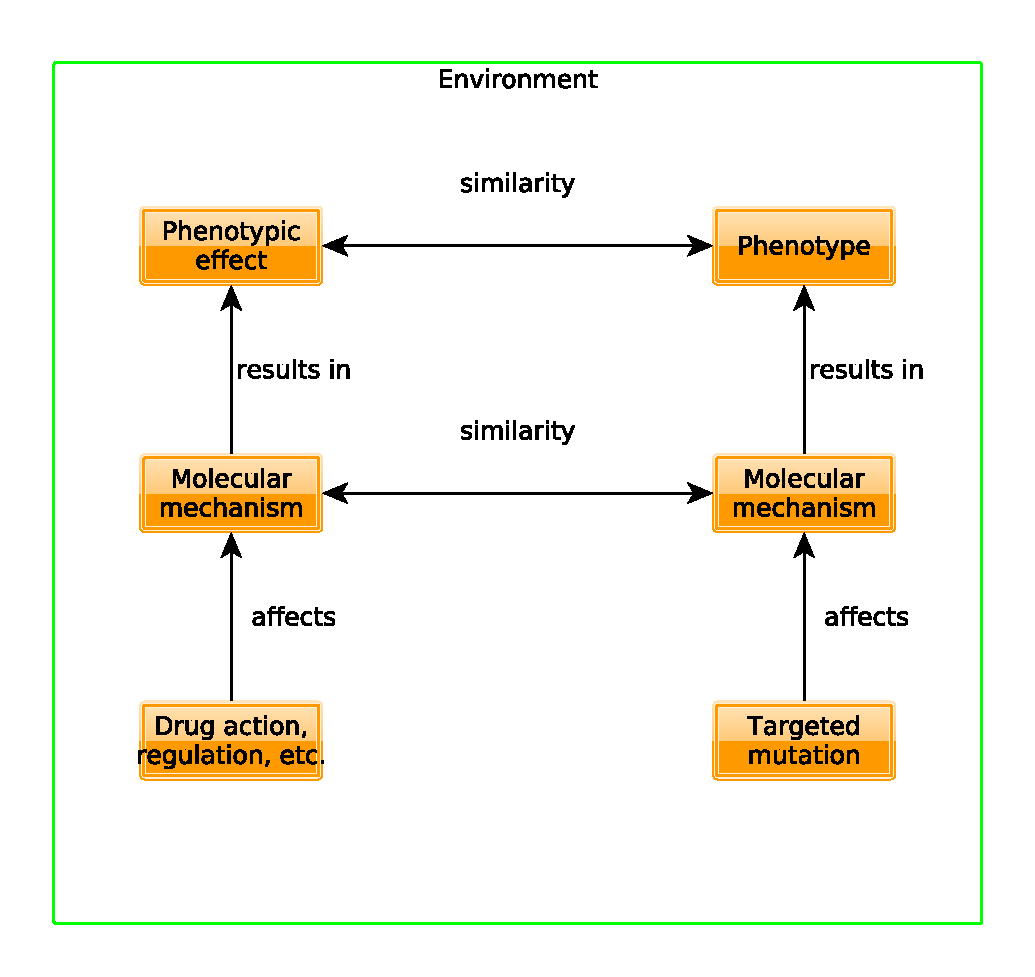
\includegraphics[height=\textheight]{similarity.eps}}
\end{frame}

\begin{frame}
  \frametitle{Applications of semantic similarity}
  \begin{itemize}
  \item Guilt-by-association:
    \begin{itemize}
    \item $x$ is associated with $y$
    \item $z$ is similar to $x$
    \item therefore: $z$ may be associated with $y$
    \end{itemize}
  \item candidate genes (polygenic disease):
    \begin{itemize}
    \item FunSimMat: similar function $\Rightarrow$ similar/same
      disease
    \item side effect similarity: similar side effects $\Rightarrow$
      similar targets/indications
    \end{itemize}
  \end{itemize}
\end{frame}

\begin{frame}
  \frametitle{Applications of semantic similarity}
  \begin{itemize}
  \item No guilt-by-association (abduction):
    \begin{itemize}
    \item $x$ causes $a$
    \item $y$ has $b$
    \item $a$ similar to $b$
    \item therefore: $b$ is caused by $x$
    \end{itemize}
  \item candidate genes (monogenic and polygenic disease):
    \begin{itemize}
    \item Phenomizer: gene $x$ causes phenotypes $a$; patient $y$ has
      symptoms $b$; $a$ is similar to $b$; therefore: gene $x$ causes
      the symptoms in $b$
    \item PhenomeNET: similar to Phenomizer but using model organism
      phenotypes (knockouts)
    \item PhenomeDrug: knockout of gene $x$ causes phenotypes $a$;
      drug $y$ causes side effects $b$; $a$ is similar to $b$;
      therefore: drug $y$ inhibits $x$ (or: phenotypes $b$ are caused
      by inhibition of $x$)
    \item needs to compare model organism phenotypes and human
      phenotypes $\Rightarrow$ ontology alignment/integration/mapping
    \end{itemize}
  \end{itemize}
\end{frame}

\begin{frame}
  \frametitle{Applications of semantic similarity}
  \begin{itemize}
  \item comparing entities annotated with {\em different}
    ontologies/vocabularies of the {\em same} (or related) domains
    \begin{itemize}
    \item medical: UMLS, HPO, DO, ORDO, NCIT, ICD, SNOMED CT, MeSH, ...
    \item phenotype: HPO, MP, CPO, WBPhenotype, FBCV, MeSH, ...
    \item chemical: ChEBI, MeSH, DrOn, RXNorm, DrugBank, ...
    \end{itemize}
  \item needs mapping, alignment, or integration
    \begin{itemize}
    \item mapping: given a term $t$, find corresponding class in
      ontology $O$
      \begin{itemize}
      \item can be 1:1, 1:n, n:1, n:m
      \item $t$ can be from ontology, vocabulary, database, or text
      \item use $O$ for analysis
      \end{itemize}
    \item alignment: given two ontologies or vocabularies $O_1$ and
      $O_2$, find all mappings between classes/terms in $O_1$ and $O_2$
      \begin{itemize}
      \item applicable to ontologies and vocabularies
      \item use $O_1$ or $O_2$ for analysis
      \end{itemize}
    \item integration: given two ontologies $O_1$ and $O_2$, combine
      both ontologies into a single ontology $O$
      \begin{itemize}
      \item maintain meaning of classes
      \item use $O$ for analysis
      \end{itemize}
    \end{itemize}
  \end{itemize}
\end{frame}

\begin{frame}
  \frametitle{Applications of semantic similarity}
  \begin{itemize}
  \item lexical mappings: use class labels (and synonyms) to find matches
    \begin{itemize}
    \item hypertension ({\tt HP:0000822}) and hypertension ({\tt MP:0000231})
    \end{itemize}
  \item semantic mappings: use class axioms to find matches
    \begin{itemize}
    \item pulmonary valve stenosis ({\tt MP:0006182}) and Pulmonic
      stenosis ({\tt HP:0001642})
    \item both definitions based on constricted ({\tt PATO:0001847})
      and pulmonary valve ({\tt UBERON:0002146})
    \end{itemize}
  \item hybrid: combine lexical and semantic mappings
  \end{itemize}
\end{frame}

\begin{frame}
  \frametitle{Applications of semantic similarity}
  tools for ontology mapping, matching, integration:
  \begin{itemize}
  \item AgreementMaker Light: \url{https://github.com/AgreementMakerLight/AML-Jar}
    \begin{itemize}
    \item structural (semantic) and lexical matches
    \item can use domain-specific background knowledge
    \end{itemize}
  \item LogMap: \url{https://github.com/ernestojimenezruiz/logmap-matcher}
    \begin{itemize}
    \item structural (semantic) and lexical matches
    \item biology-themed versions
    \end{itemize}
  \item NCBO Annotator: \url{https://bioportal.bioontology.org/annotator}
    \begin{itemize}
    \item lexical matches only
    \item can annotate full text
    \end{itemize}
  \item recent tools and comprehensive ongoing evaluation:
    \begin{itemize}
    \item OAEI: \url{http://oaei.ontologymatching.org/}
    \end{itemize}
  \end{itemize}
\end{frame}

\begin{frame}
  \frametitle{Applications of semantic similarity}
  semantic similarity and text mining:
  \begin{itemize}
  \item find all occurrences of classes of one (or more) ontologies in text
    \begin{itemize}
    \item using lexical matching or semantic annotations
      of text
    \item TextPresso (\url{http://www.textpresso.org/}), NCBO
      Annotator (\url{https://bioportal.bioontology.org/annotator}),
      WhatIzIt (\url{http://www.ebi.ac.uk/webservices/whatizit/info.jsf})
    \item ontology-specific text normalization tools
      \begin{itemize}
      \item DNorm (diseases), GNorm (gene names), OSCAR (chemicals), ...
      \end{itemize}
    \end{itemize}
  \item use for database construction (automatic annotation), relation
    extraction, network construction (co-occurrence network), etc.
  \end{itemize}
\end{frame}

% \begin{frame}
%   \frametitle{Applications of semantic similarity}
%   \centerline{http://aber-owl.net/aber-owl/diseasephenotypes/}
%   \begin{itemize}
%   \item find phenotypes (signs and symptoms) associated with common
%     diseases
%     \begin{itemize}
%     \item no resource available for comparison
%     \end{itemize}
%   \item pattern-based mining of literature with Aber-OWL: PubMed
%   \item evaluation (of genetically based disease phenotypes) with
%     experimentally validated disease genes
%   \end{itemize}
% \end{frame}

% \begin{frame}
%   \frametitle{Applications of semantic similarity}
%   \framesubtitle{http://aber-owl.net/aber-owl/diseasephenotypes/}
%   \centerline{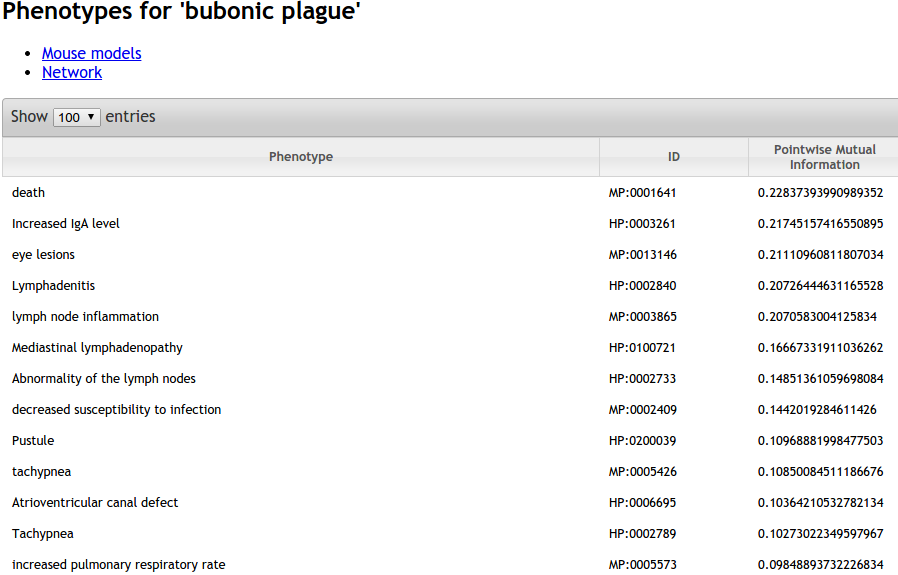
\includegraphics[width=1\textwidth]{aber-owl-plague.png}}
% \end{frame}

% \begin{frame}
%   \frametitle{Applications of semantic similarity}
%   \framesubtitle{http://aber-owl.net/aber-owl/diseasephenotypes/}
%   \centerline{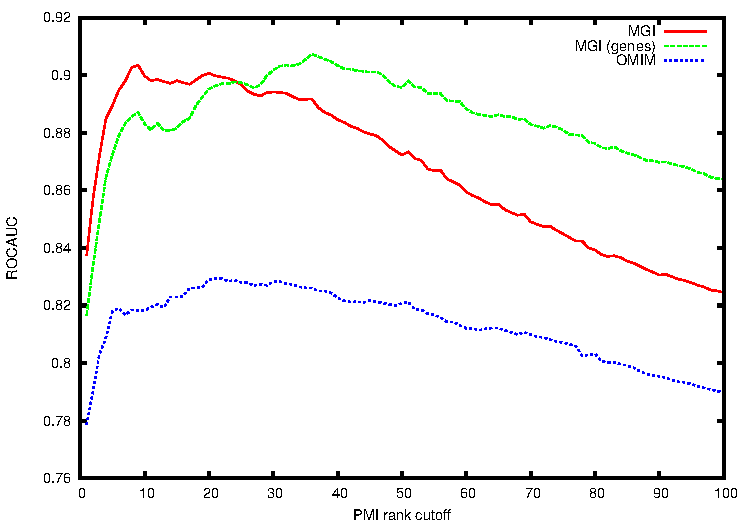
\includegraphics[width=1\textwidth]{pmi-auc-plot.pdf}}
% \end{frame}

% \begin{frame}[plain]
%   \frametitle{Applications of semantic similarity}
%   \centerline{\includegraphics[height=1\textheight]{network.eps}}
% \end{frame}

\begin{frame}
  \frametitle{Applications of semantic similarity}
  \begin{itemize}
  \item semantic similarity can be used as features in machine
    learning models
    \begin{itemize}
    \item when annotation space is too large
      \begin{itemize}
      \item e.g., GO: 50,000 classes
      \item replace binary representation
      \end{itemize}
    \item to incorporate background knowledge
      \begin{itemize}
      \item semantic similarity encodes {\em implicitly} for ontology
        structure and axioms
      \item encodes for {\em specificity} of classes
      \end{itemize}
    \item negative: reduce all annotations to single value
      \begin{itemize}
      \item leads to loss of information
      \item but is easier to use by many machine learning methods
      \end{itemize}
    \end{itemize}
  \end{itemize}
\end{frame}

% \begin{frame}
%   \frametitle{Applications of semantic similarity}
%   \begin{tikzpicture}[remember picture,overlay]
%     \node[at=(current page.center)] {
%       \centerline{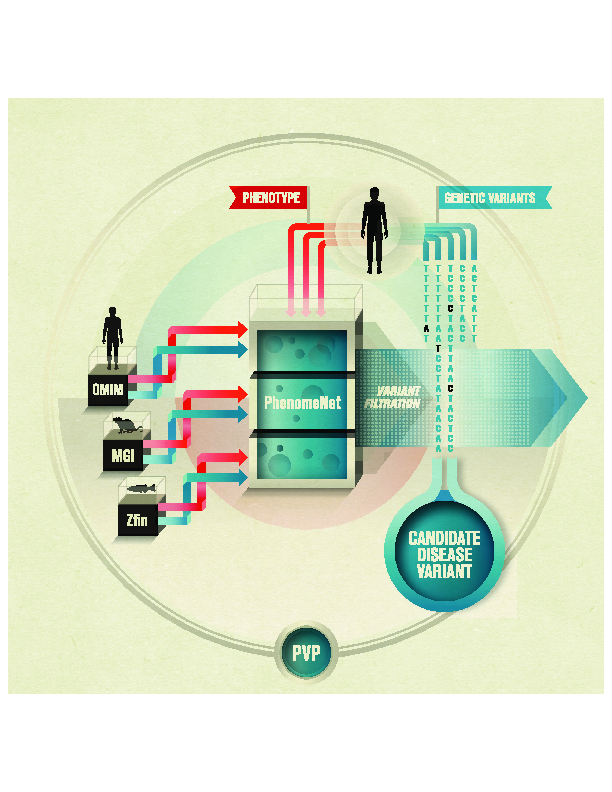
\includegraphics[height=1\textheight]{pvp.pdf}}
%     };
%   \end{tikzpicture}
% \end{frame}

% {
% \setbeamercolor{background canvas}{bg=}
% 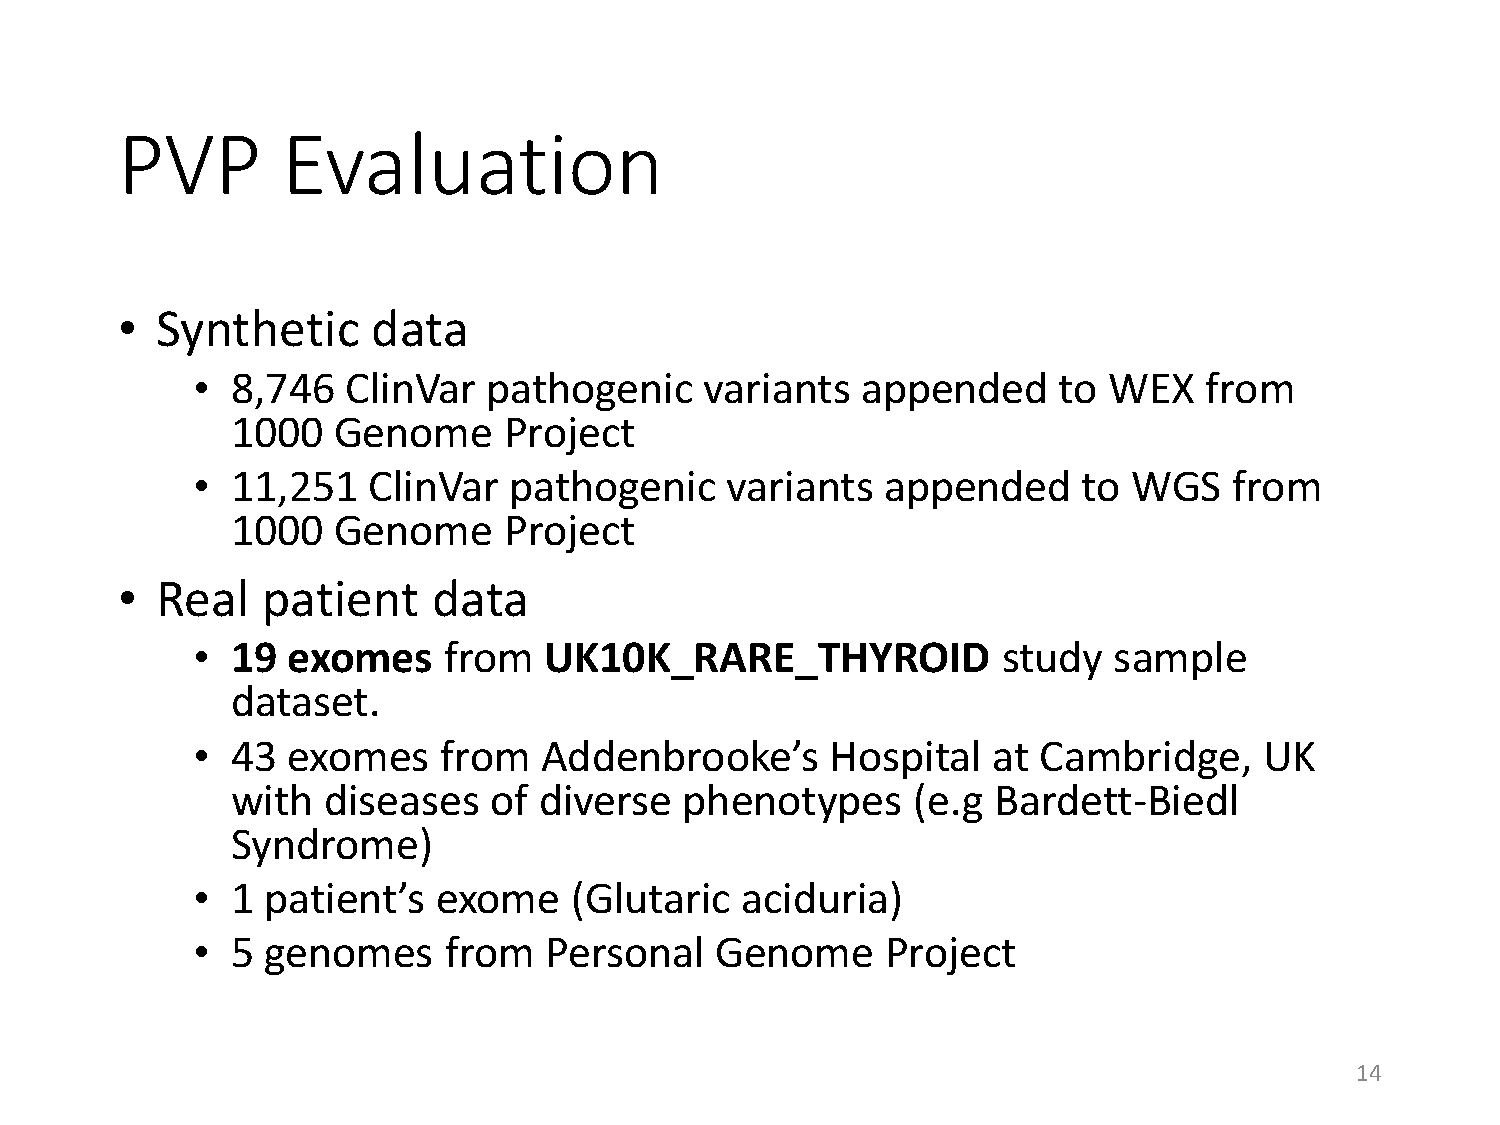
\includepdf[pages=1-3]{hh-pvp2.pdf}
% }

\begin{frame}
  \frametitle{Summary}
  \begin{itemize}
  \item many semantic similarity measures
    \begin{itemize}
    \item graph-based
    \item feature-based
    \end{itemize}
  \item useful for similarity-based prediction
    \begin{itemize}
    \item similar entities $\Rightarrow$ guilt-by-association
    \item different entities
    \end{itemize}
  \item combine with data and text mining
  \item features in machine learning methods
  \end{itemize}
\end{frame}

\begin{frame}
  \frametitle{Acknowledgements}
  \begin{itemize}
  \item Sarah Alghamdi
  \item Mona Alsharani
  \item Imene Boudellioua
  \item Senay Kafkas
  \item Maxat Kulmanov
  \item Fatima Zohra Smaili
  \end{itemize}
\end{frame}

\begin{frame}
  \frametitle{Hands-on: semantic similarity}
  \begin{itemize}
  \item if you have not done so {\em before} the tutorial, don't start
    now
    \begin{itemize}
    \item you need to download {\em a lot} of data
    \item you can just follow our demonstration and try later
    \item (unless Internet is exceptionally fast for a conference
      Wifi, then just go ahead and do everything now)
    \end{itemize}
  \item Jupyter Notebook
    \begin{itemize}
    \item notebooks consist of code and rich text fragments
    \item human readable (with nice figures) {\em and} executable
    \item need to install the SciJava kernel (default: iPython)
    \item very widely used
    \end{itemize}
  \item
    \url{https://github.com/bio-ontology-research-group/ontology-tutorial}
  \end{itemize}
\end{frame}

\begin{frame}
  \frametitle{Hands-on: semantic similarity}
  In the tutorial, we will
  \begin{itemize}
  \item download an ontology
  \item explore the ontology with OWLAPI
  \item classify the ontology with an OWL reasoner
    \begin{itemize}
    \item and query using an OWL reasoner
    \end{itemize}
  \item store the inferred version locally
  \item use the Semantic Measures Library to:
    \begin{itemize}
    \item explore the ontology as graph
    \item compute similarity between classes
    \item use different similarity measures
    \item compare patients to mice
    \end{itemize}
  \item learn to use Onto2Vec and OPA2Vec
  \item you can build on this and extend for your own research!
  \end{itemize}
\end{frame}

\begin{frame}
  \frametitle{Hands-on: semantic similarity}
  Do the tutorial...
\end{frame}

\begin{frame}
  \frametitle{Hands-on: semantic similarity}
  \begin{itemize}
  \item now play with the Notebook:
    \begin{itemize}
    \item look at the results list (check MGI)
    \item try another disease (check OMIM)
    \item or a drug effect (check SIDER)
    \end{itemize}
  \item you can also test another ontology
    \begin{itemize}
    \item GO for functional similarity
    \item ChEBI for chemical (structural) similarity
    \item or yeast phenotypes
    \end{itemize}
  \end{itemize}
\end{frame}

\end{document}
%%% Local Variables:
%%% mode: latex
%%% TeX-master: t
%%% End:
